\documentclass[9pt]{beamer}
\usetheme{Madrid}
\usepackage{mathtools}
\usepackage{bm}
\usepackage{esvect}
\usepackage{amsmath}
\usepackage{physics}
\usepackage{empheq}
\usepackage[many]{tcolorbox}

%$\vv{\bm{L}}

\title{Are neutrinos their own antiparticles?}
 
\subtitle{What do we talk about when we talk about neutrinos?}
 
\author{J.J. G\'omez Cadenas}
 
\institute{Donostia International Physics Center (DIPC)} % (optional)
 
\date[October 6th, 2018] % (optional)
{PHYSIS, SAN SEBASTIAN: 2-6 OCTOBER 2018}
 
\logo{
\includegraphics[height=0.5cm]{dipc.png}

\includegraphics[height=0.5cm]{IB.png}}


\tcbset{highlight math style={enhanced,
  colframe=red!60!black,colback=yellow!50!white,arc=4pt,boxrule=1pt,
  }}

\newtcbox{\mybox}[1][]{nobeforeafter,math upper,tcbox raise base,
  enhanced,frame hidden,boxrule=0pt,interior style={top color=green!10!white,
  bottom color=green!10!white,middle color=green!50!yellow},
  fuzzy halo=1pt with green,drop large lifted shadow,#1}
\begin{document}

\frame{\titlepage}

%\begin{frame}
\frametitle{The continuous beta spectrum}

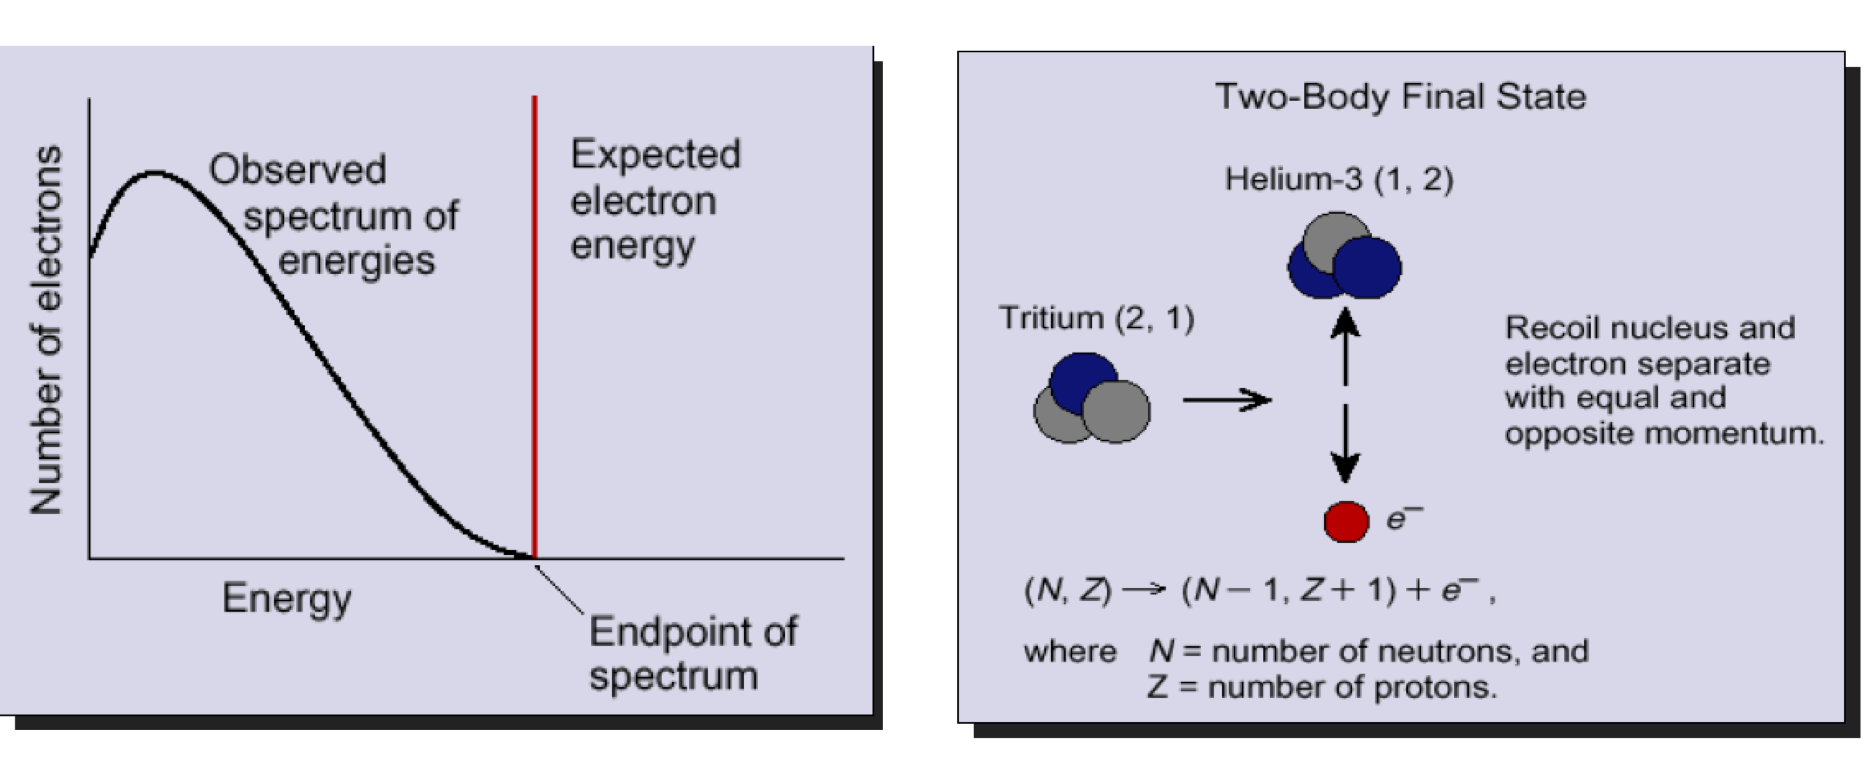
\includegraphics[scale=0.38]{pool/imgTalks/beta-ray.png}
 
\end{frame}
%


\begin{frame}
\frametitle{Liebe Radioaktive Damen und Herren}
\begin{columns}
 
\column{0.5\textwidth}
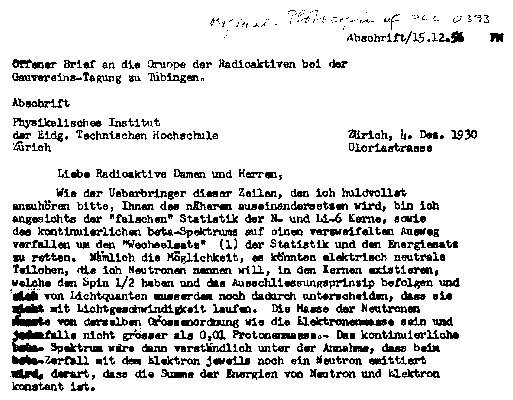
\includegraphics[scale=0.4]{liebe.png}
 
\column{0.2\textwidth}
\begin{block}{}
Dear Radioactive Ladies and Getlemen.

...because the continuous beta spectrum...I have hit upon a desperate remedy to save the law of conservation of energy.

\end{block}
\end{columns}
\end{frame}


%\begin{frame}
\frametitle{Why so desperate?}


\includegraphics[scale=0.4]{desperate.png}
 

\begin{block}{}
Because conservation of energy-momentum means that physics does not depend on space-time translations. We believe that physics laws must be the same here than in Andromeda, and the same today than next or last year. Physicists, then, could not give up on energy conservation.

\end{block}

\end{frame}

%\begin{frame}
\frametitle{Two and three body kinematics}

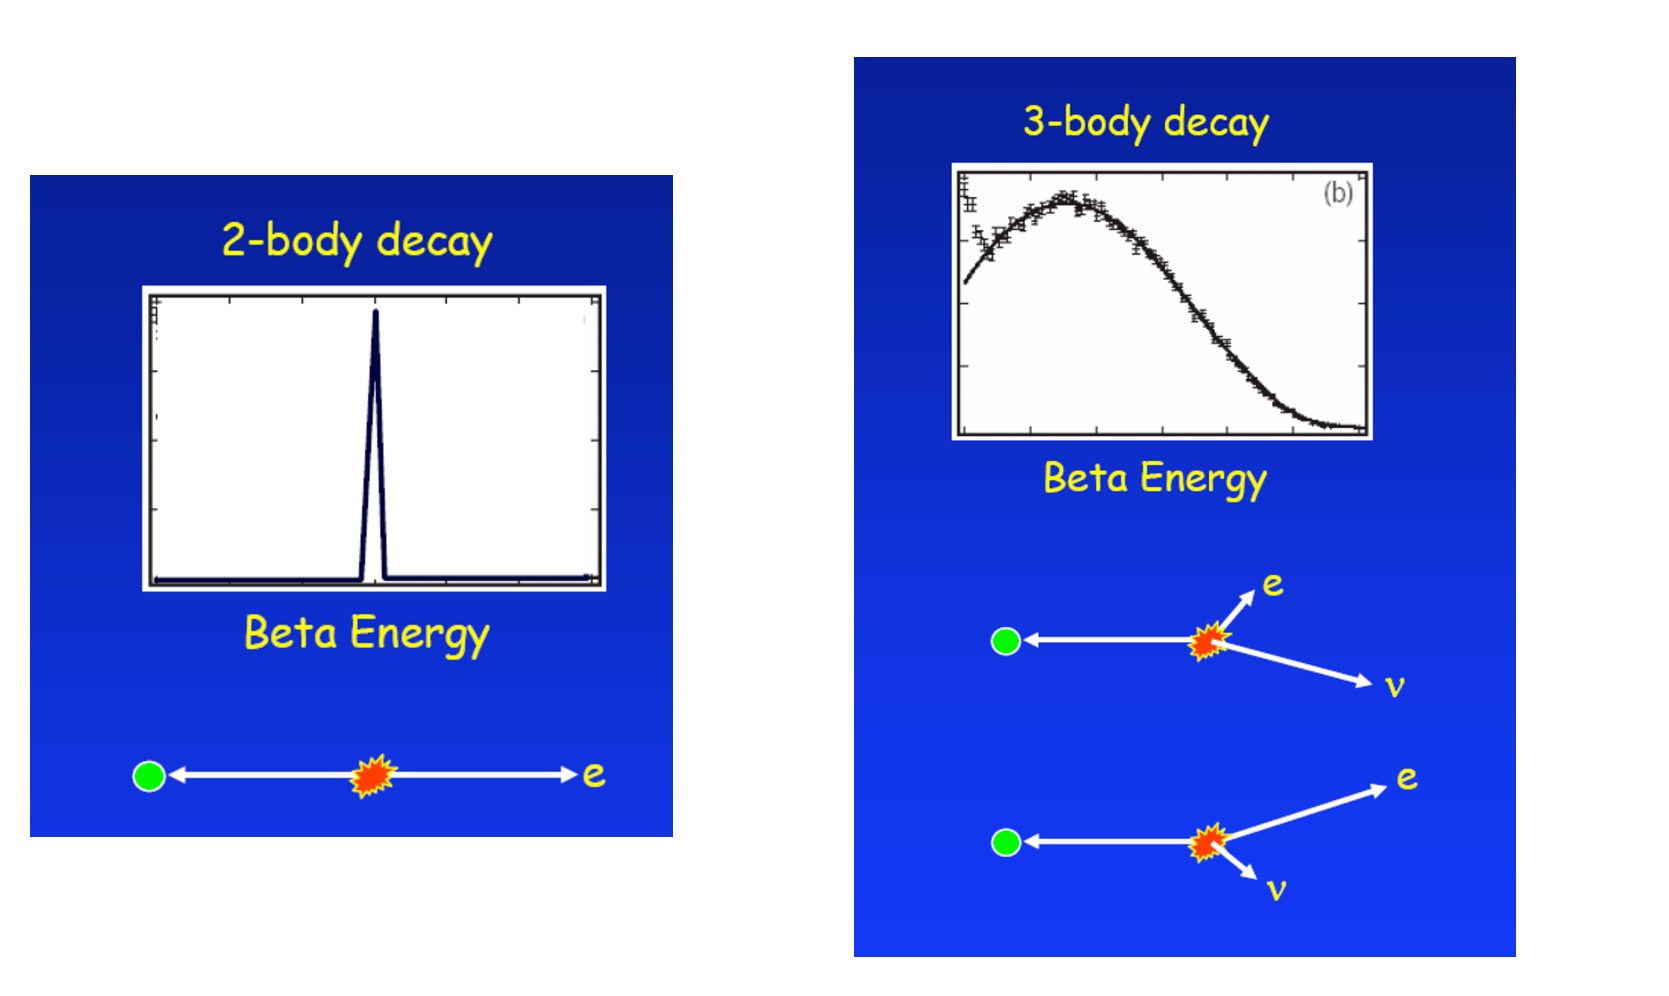
\includegraphics[scale=0.4]{kinematics.pdf}
 
\end{frame}

%\begin{frame}
\frametitle{Pauli's neutrino}
\begin{columns}
\column{0.45\textwidth}
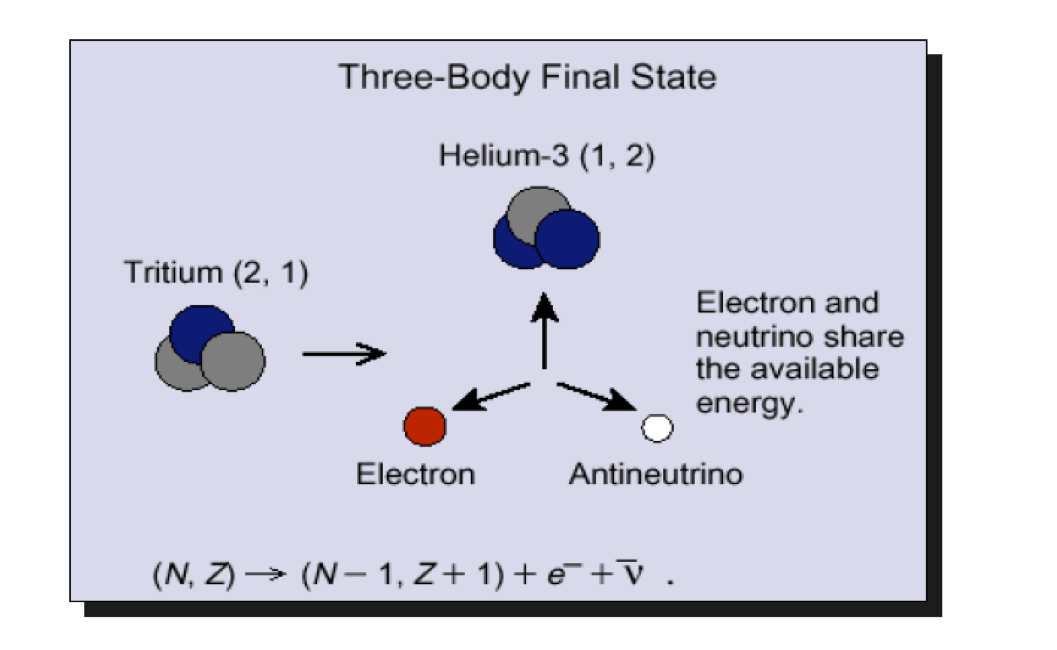
\includegraphics[scale=0.4]{pauli-neutrino.png}
 
 \column{0.3\textwidth}
\begin{block}{}
{\bf Electrically neutral particles which have spin 1/2 and obey the exclusion principle... the mass should be of the order of the electron mass}. In other words, Pauli ``neutrons''  were nothing but neutral electrons. 
\end{block}
\end{columns}
\end{frame}

%\begin{frame}
\frametitle{I have done a terrible thing}

\begin{columns}
\column{0.35\textwidth}
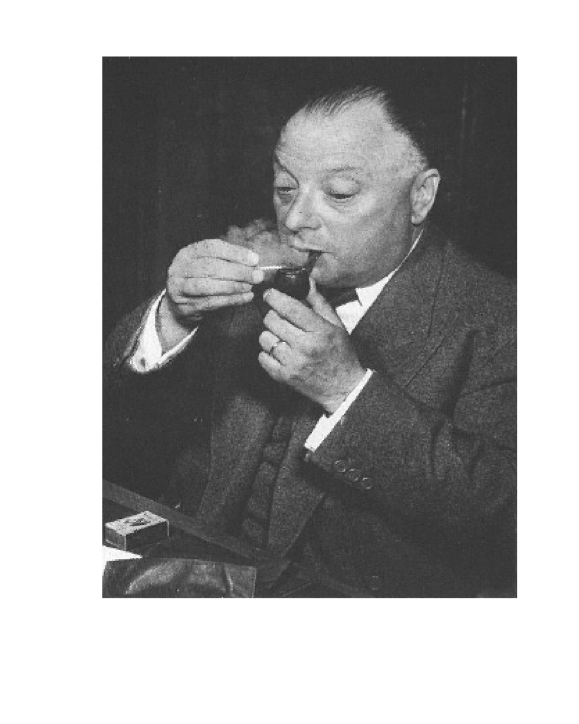
\includegraphics[scale=0.3]{pauli.png}
 
 \column{0.4\textwidth}
\begin{block}{}
Pauli neutral particles had to interact very weakly in order to escape undetected. Furthermore the mechanism by which the ``neutron" was produced was unspecified.

\vspace{0.5cm}

Pauli was unhappy with his brainchild. We wrote: ``I have  done a terrible thing. I have proposed a particle that cannot be detected. It is something no theorist should ever do". 

\end{block}
\end{columns}
\end{frame}

%\begin{frame}
\frametitle{I do not believe in neutrinos}
\begin{columns}
\column{0.35\textwidth}
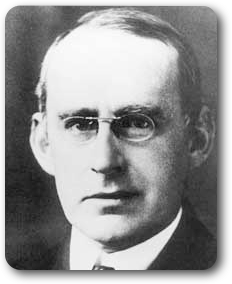
\includegraphics[scale=0.3]{eddington.png}
 
 \column{0.6\textwidth}
%\begin{block}{}
Sir Arthur Eddington: ``Just now nuclear physicists are writing a great deal about hypothetical particles called neutrinos supposed to account for certain peculiar facts observed in $\beta$-ray disintegration. We can perhaps best describe the neutrinos as little bits of spin-energy that have got detached. I am not much impressed by the neutrino theory. In an ordinary way I might say that I do not believe in neutrinos... But I have to reflect that a physicist may be an artist, and you never know where you are with artists. My old-fashioned kind of disbelief in neutrinos is scarcely enough. Dare I say that experimental physicists will not have sufficient ingenuity to make neutrinos?"

%\end{block}
\end{columns}
\end{frame}

%\begin{frame}
\frametitle{The neutron becomes the neutrino}
\begin{columns}
\column{0.35\textwidth}
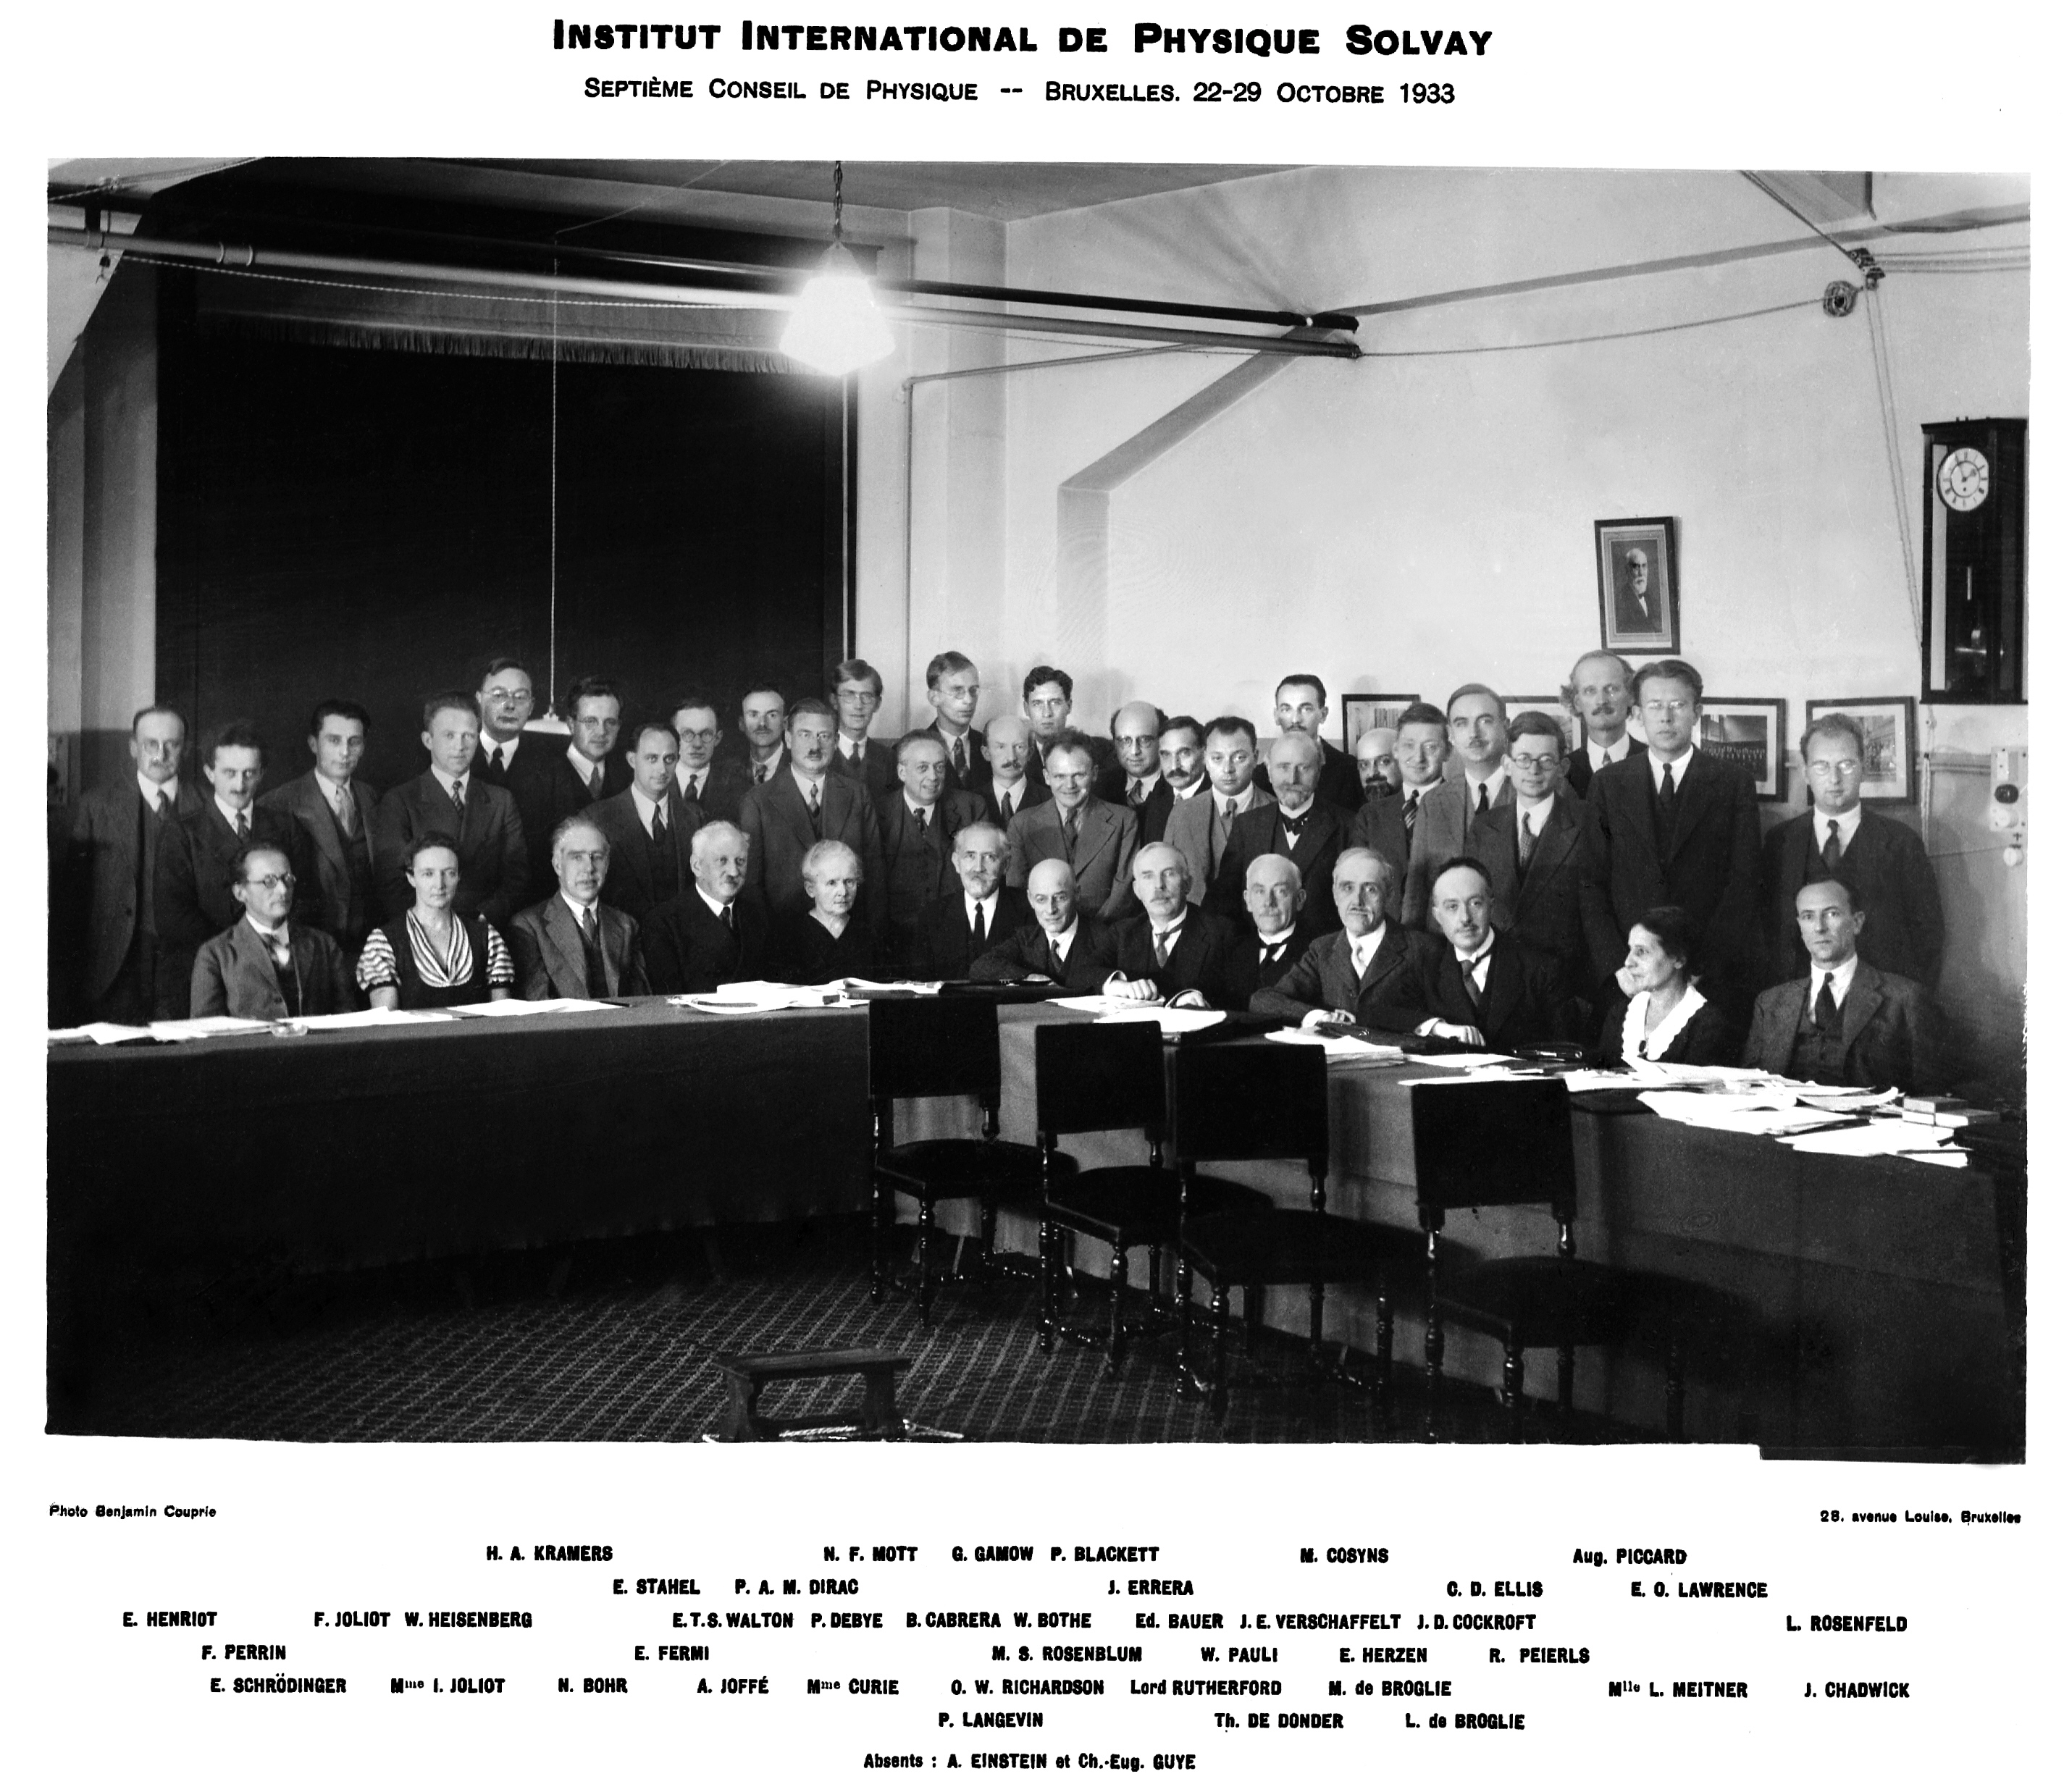
\includegraphics[scale=0.18]{Solvay1933Large.jpg}
 
 \column{0.6\textwidth}
%\begin{block}{}
Pauli in  1933 at the Solvay Congress: ``Regarding the properties of these neutral particles, the atomic weights
of the radioactive elements tell us first of all that their mass cannot exceed
much that of the electron. In order to distinguish them from the heavy
neutrons, Mr. Fermi proposed the name ``neutrino.'' {\bf It's possible that the
neutrinos' own mass might be equal to zero, so that they would have to
propagate with the speed of light, like the photons}. However, their penetrating power would exceed by far that of photons of the same energy. It
seems to me acceptable that the neutrinos have spin 1/2 and satisfy Fermi's 
statistics, although experiments do not give us any direct proof of this hypothesis. 
{\bf We know nothing about the interaction of the neutrinos with other material particles and with the photons".}

%\end{block}
\end{columns}
\end{frame}

\begin{frame}
\frametitle{The continuous beta spectrum}

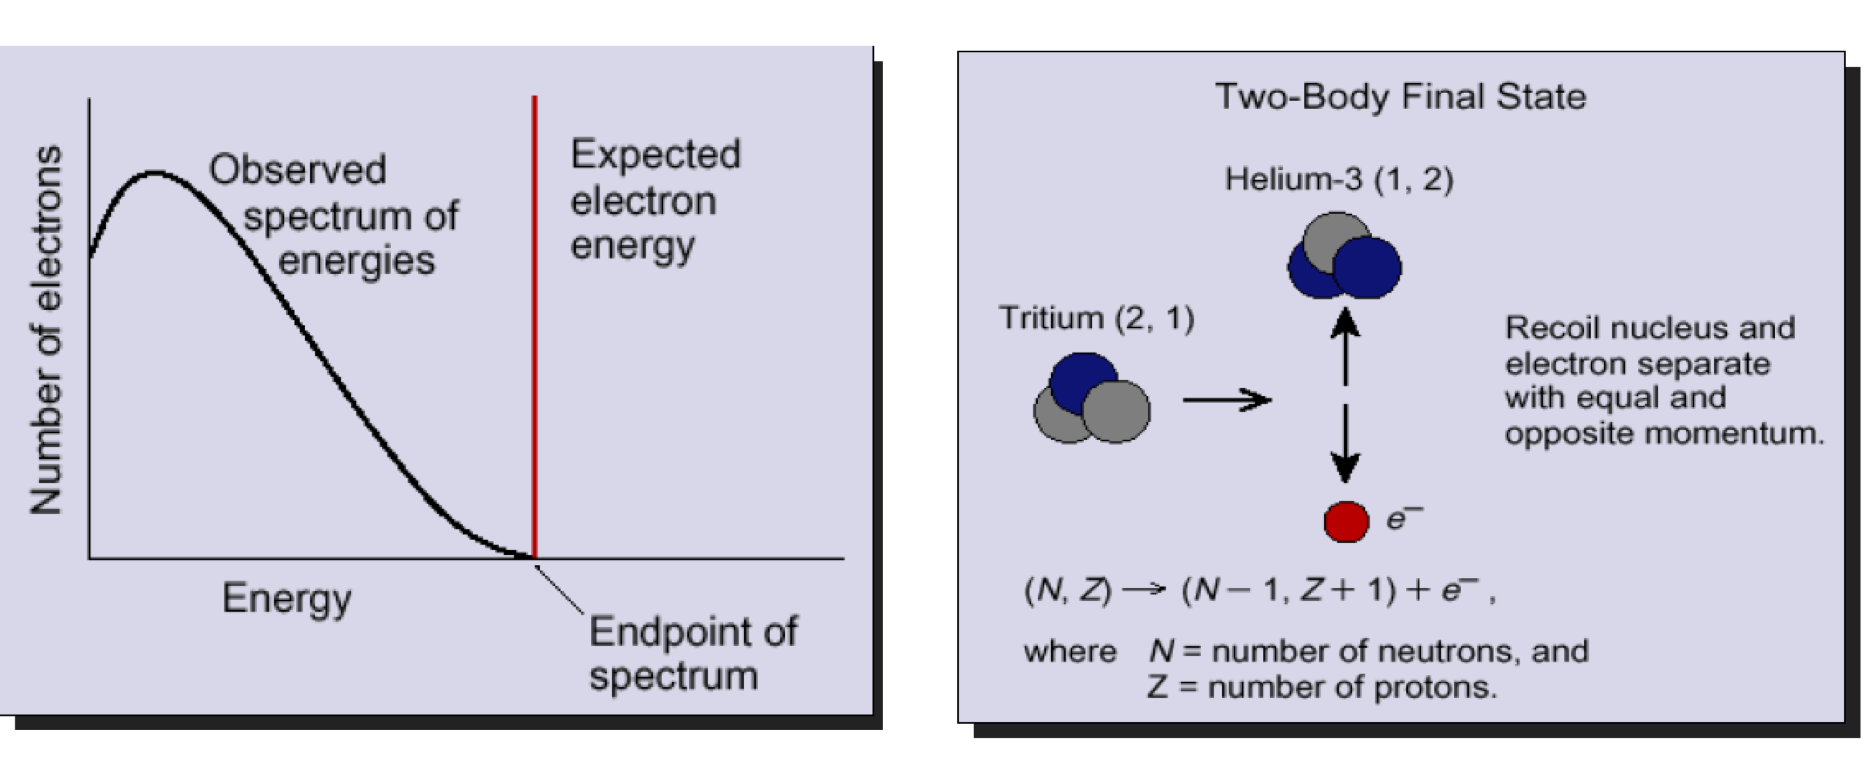
\includegraphics[scale=0.38]{pool/imgTalks/beta-ray.png}
 
\end{frame}


\begin{frame}
\frametitle{Liebe Radioaktive Damen und Herren}
\begin{columns}
 
\column{0.5\textwidth}
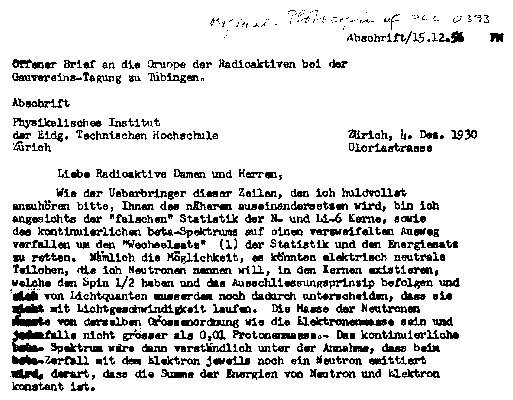
\includegraphics[scale=0.4]{liebe.png}
 
\column{0.2\textwidth}
\begin{block}{}
Dear Radioactive Ladies and Getlemen.

...because the continuous beta spectrum...I have hit upon a desperate remedy to save the law of conservation of energy.

\end{block}
\end{columns}
\end{frame}


\begin{frame}
\frametitle{Why so desperate?}


\includegraphics[scale=0.4]{desperate.png}
 

\begin{block}{}
Because conservation of energy-momentum means that physics does not depend on space-time translations. We believe that physics laws must be the same here than in Andromeda, and the same today than next or last year. Physicists, then, could not give up on energy conservation.

\end{block}

\end{frame}

\begin{frame}
\frametitle{Two and three body kinematics}

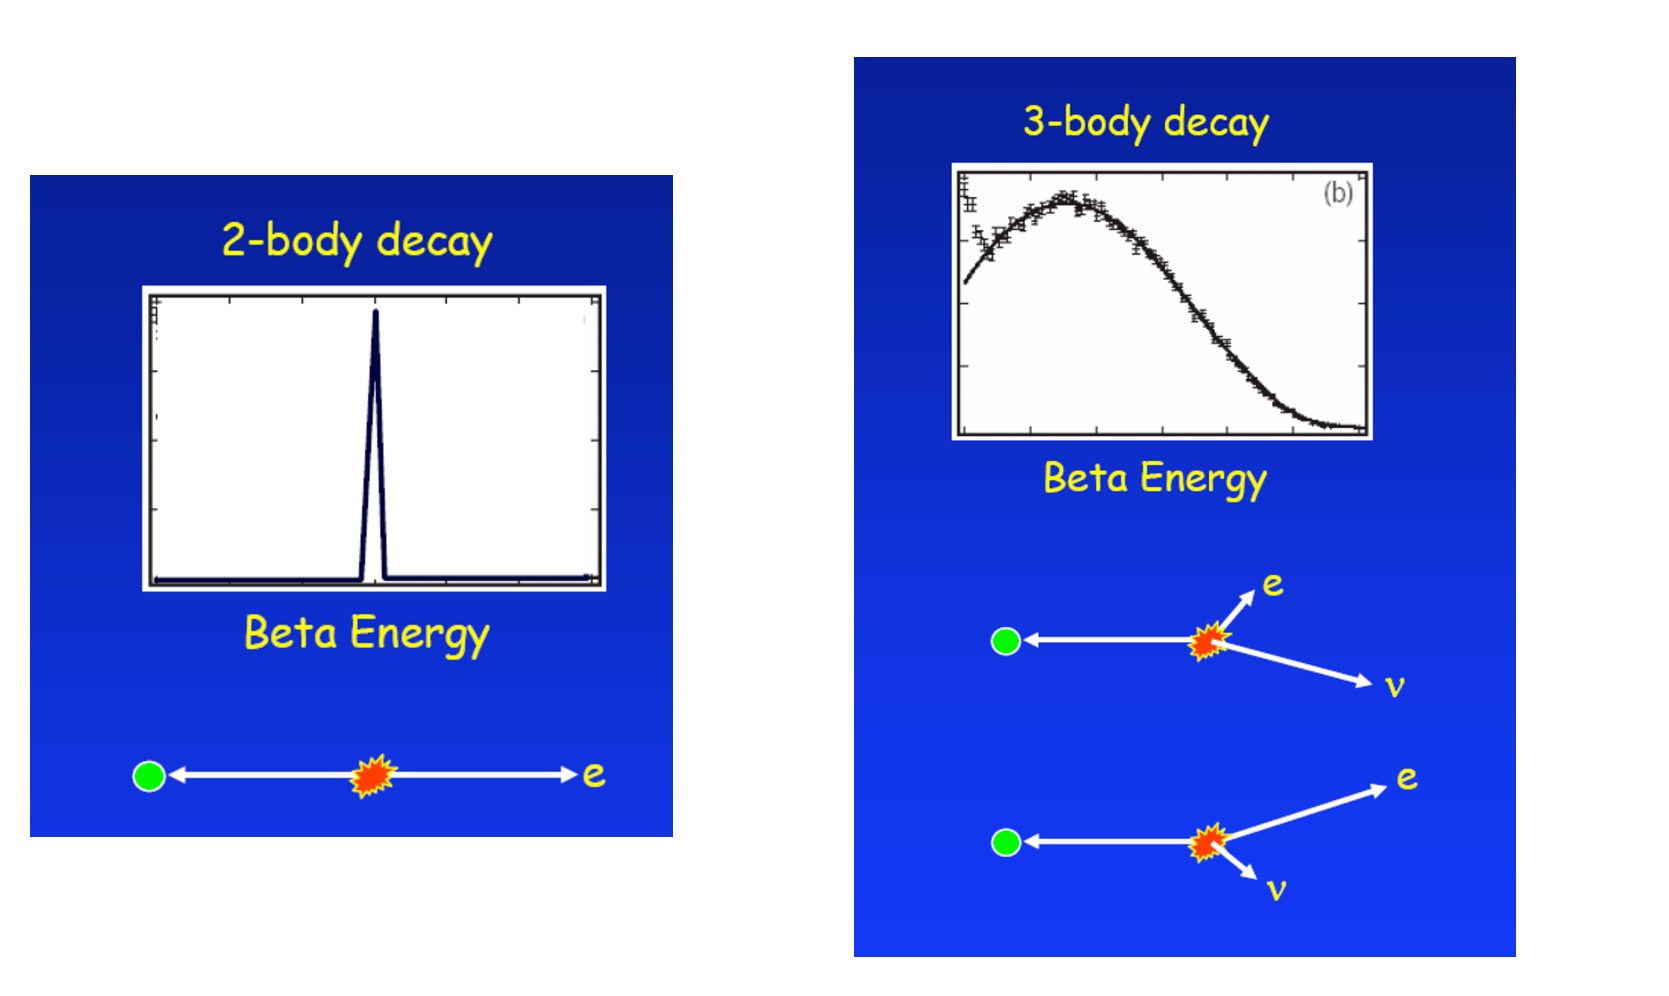
\includegraphics[scale=0.4]{kinematics.pdf}
 
\end{frame}

\begin{frame}
\frametitle{Pauli's neutrino}
\begin{columns}
\column{0.35\textwidth}
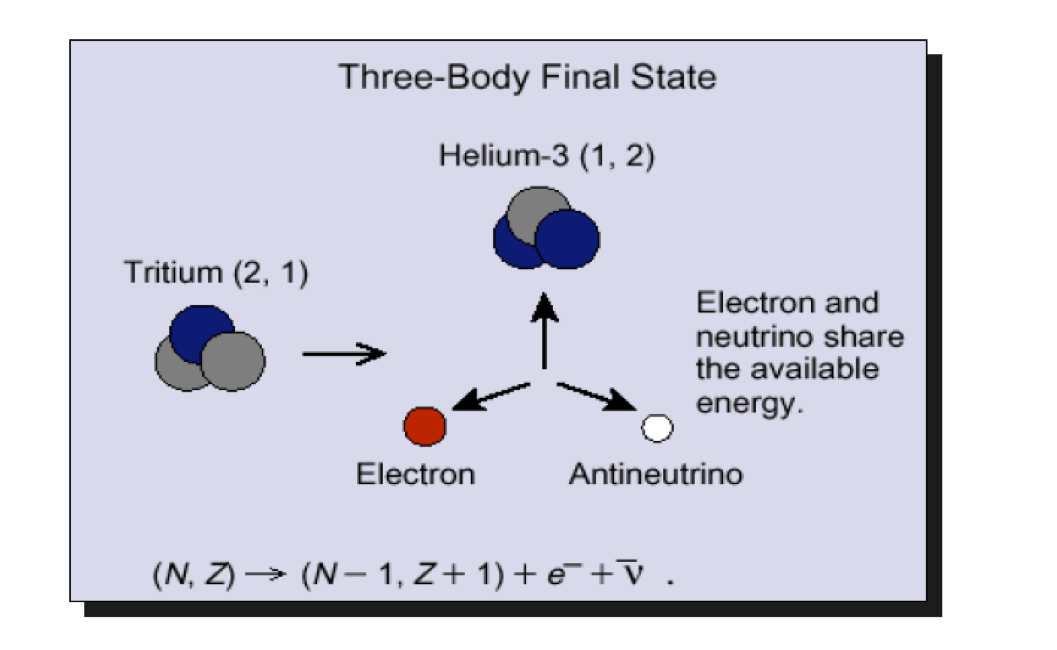
\includegraphics[scale=0.3]{pauli-neutrino.png}

\noindent Pauli in  1933 at the Solvay Congress: 

Regarding the properties of these neutral particles, the atomic weights
of the radioactive elements tell us first of all that their mass cannot exceed
much that of the electron.

 \column{0.50\textwidth}
 In order to distinguish them from the heavy
neutrons, Mr. Fermi proposed the name ``neutrino.'' {\bf It's possible that the
neutrinos' own mass might be equal to zero, so that they would have to
propagate with the speed of light, like the photons}. However, their penetrating power would exceed by far that of photons of the same energy. It
seems to me acceptable that the neutrinos have spin 1/2 and satisfy Fermi's 
statistics, although experiments do not give us any direct proof of this hypothesis. 
{\bf We know nothing about the interaction of the neutrinos with other material particles and with the photons".}
\end{columns}
\end{frame}

%\begin{frame}
%\frametitle{Pauli's neutrino}
%\begin{columns}
%\column{0.45\textwidth}
%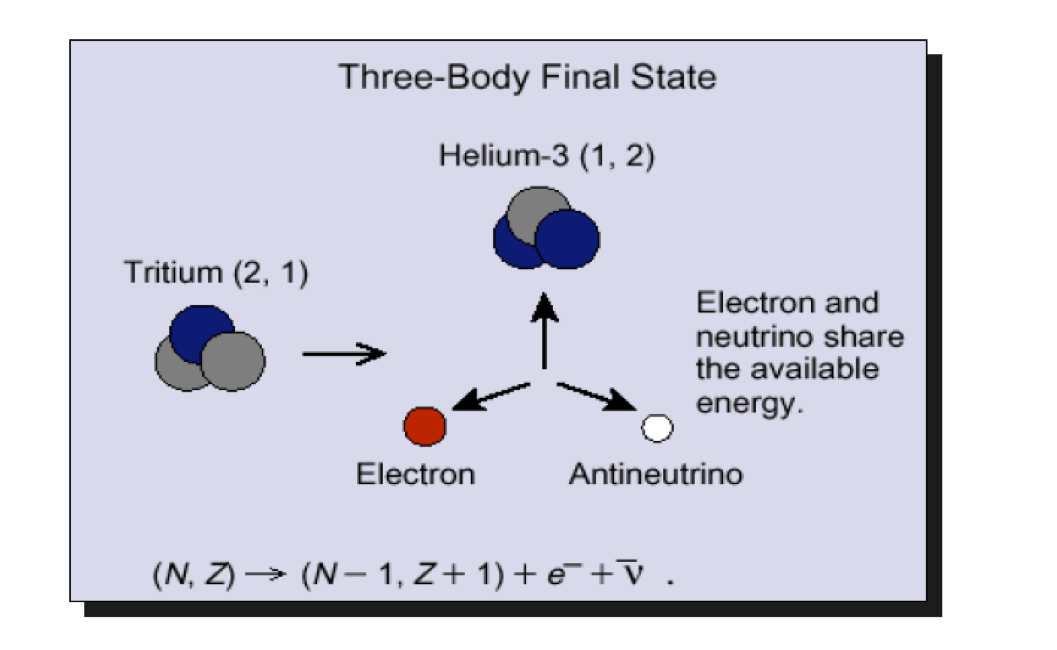
\includegraphics[scale=0.4]{pauli-neutrino.png}
% 
% \column{0.3\textwidth}
%\begin{block}{}
%{\bf Electrically neutral particles which have spin 1/2 and obey the exclusion principle... the mass should be of the order of the electron mass}. 
%\end{block}
%\end{columns}
%\end{frame}

%\begin{frame}
%\frametitle{I have done a terrible thing}
%
%\begin{columns}
%\column{0.35\textwidth}
%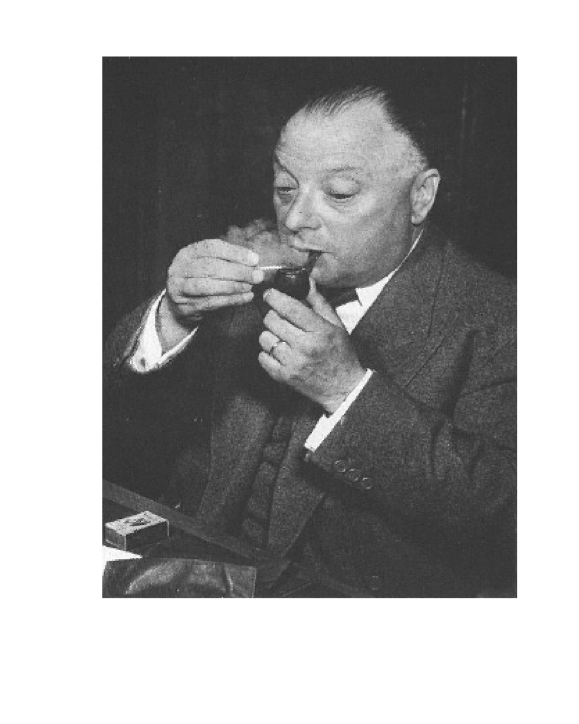
\includegraphics[scale=0.3]{pauli.png}
% 
% \column{0.4\textwidth}
%\begin{block}{}
%Pauli neutral particles had to interact very weakly in order to escape undetected. Furthermore the mechanism by which the ``neutron" was produced was unspecified.
%
%\vspace{0.5cm}
%
%Pauli was unhappy with his brainchild. We wrote: ``I have  done a terrible thing. I have proposed a particle that cannot be detected. It is something no theorist should ever do". 
%
%\end{block}
%\end{columns}
%\end{frame}

%\begin{frame}
%\frametitle{I do not believe in neutrinos}
%\begin{columns}
%\column{0.35\textwidth}
%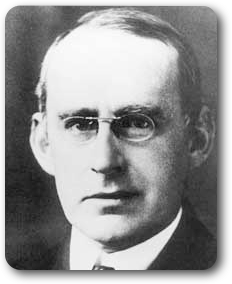
\includegraphics[scale=0.3]{eddington.png}
% 
% \column{0.6\textwidth}
%%\begin{block}{}
%Sir Arthur Eddington: ``Just now nuclear physicists are writing a great deal about hypothetical particles called neutrinos supposed to account for certain peculiar facts observed in $\beta$-ray disintegration. We can perhaps best describe the neutrinos as little bits of spin-energy that have got detached. I am not much impressed by the neutrino theory. In an ordinary way I might say that I do not believe in neutrinos... But I have to reflect that a physicist may be an artist, and you never know where you are with artists. My old-fashioned kind of disbelief in neutrinos is scarcely enough. Dare I say that experimental physicists will not have sufficient ingenuity to make neutrinos?"
%
%%\end{block}
%\end{columns}
%\end{frame}

%\begin{frame}
%\frametitle{The neutron becomes the neutrino}
%\begin{columns}
%\column{0.35\textwidth}
%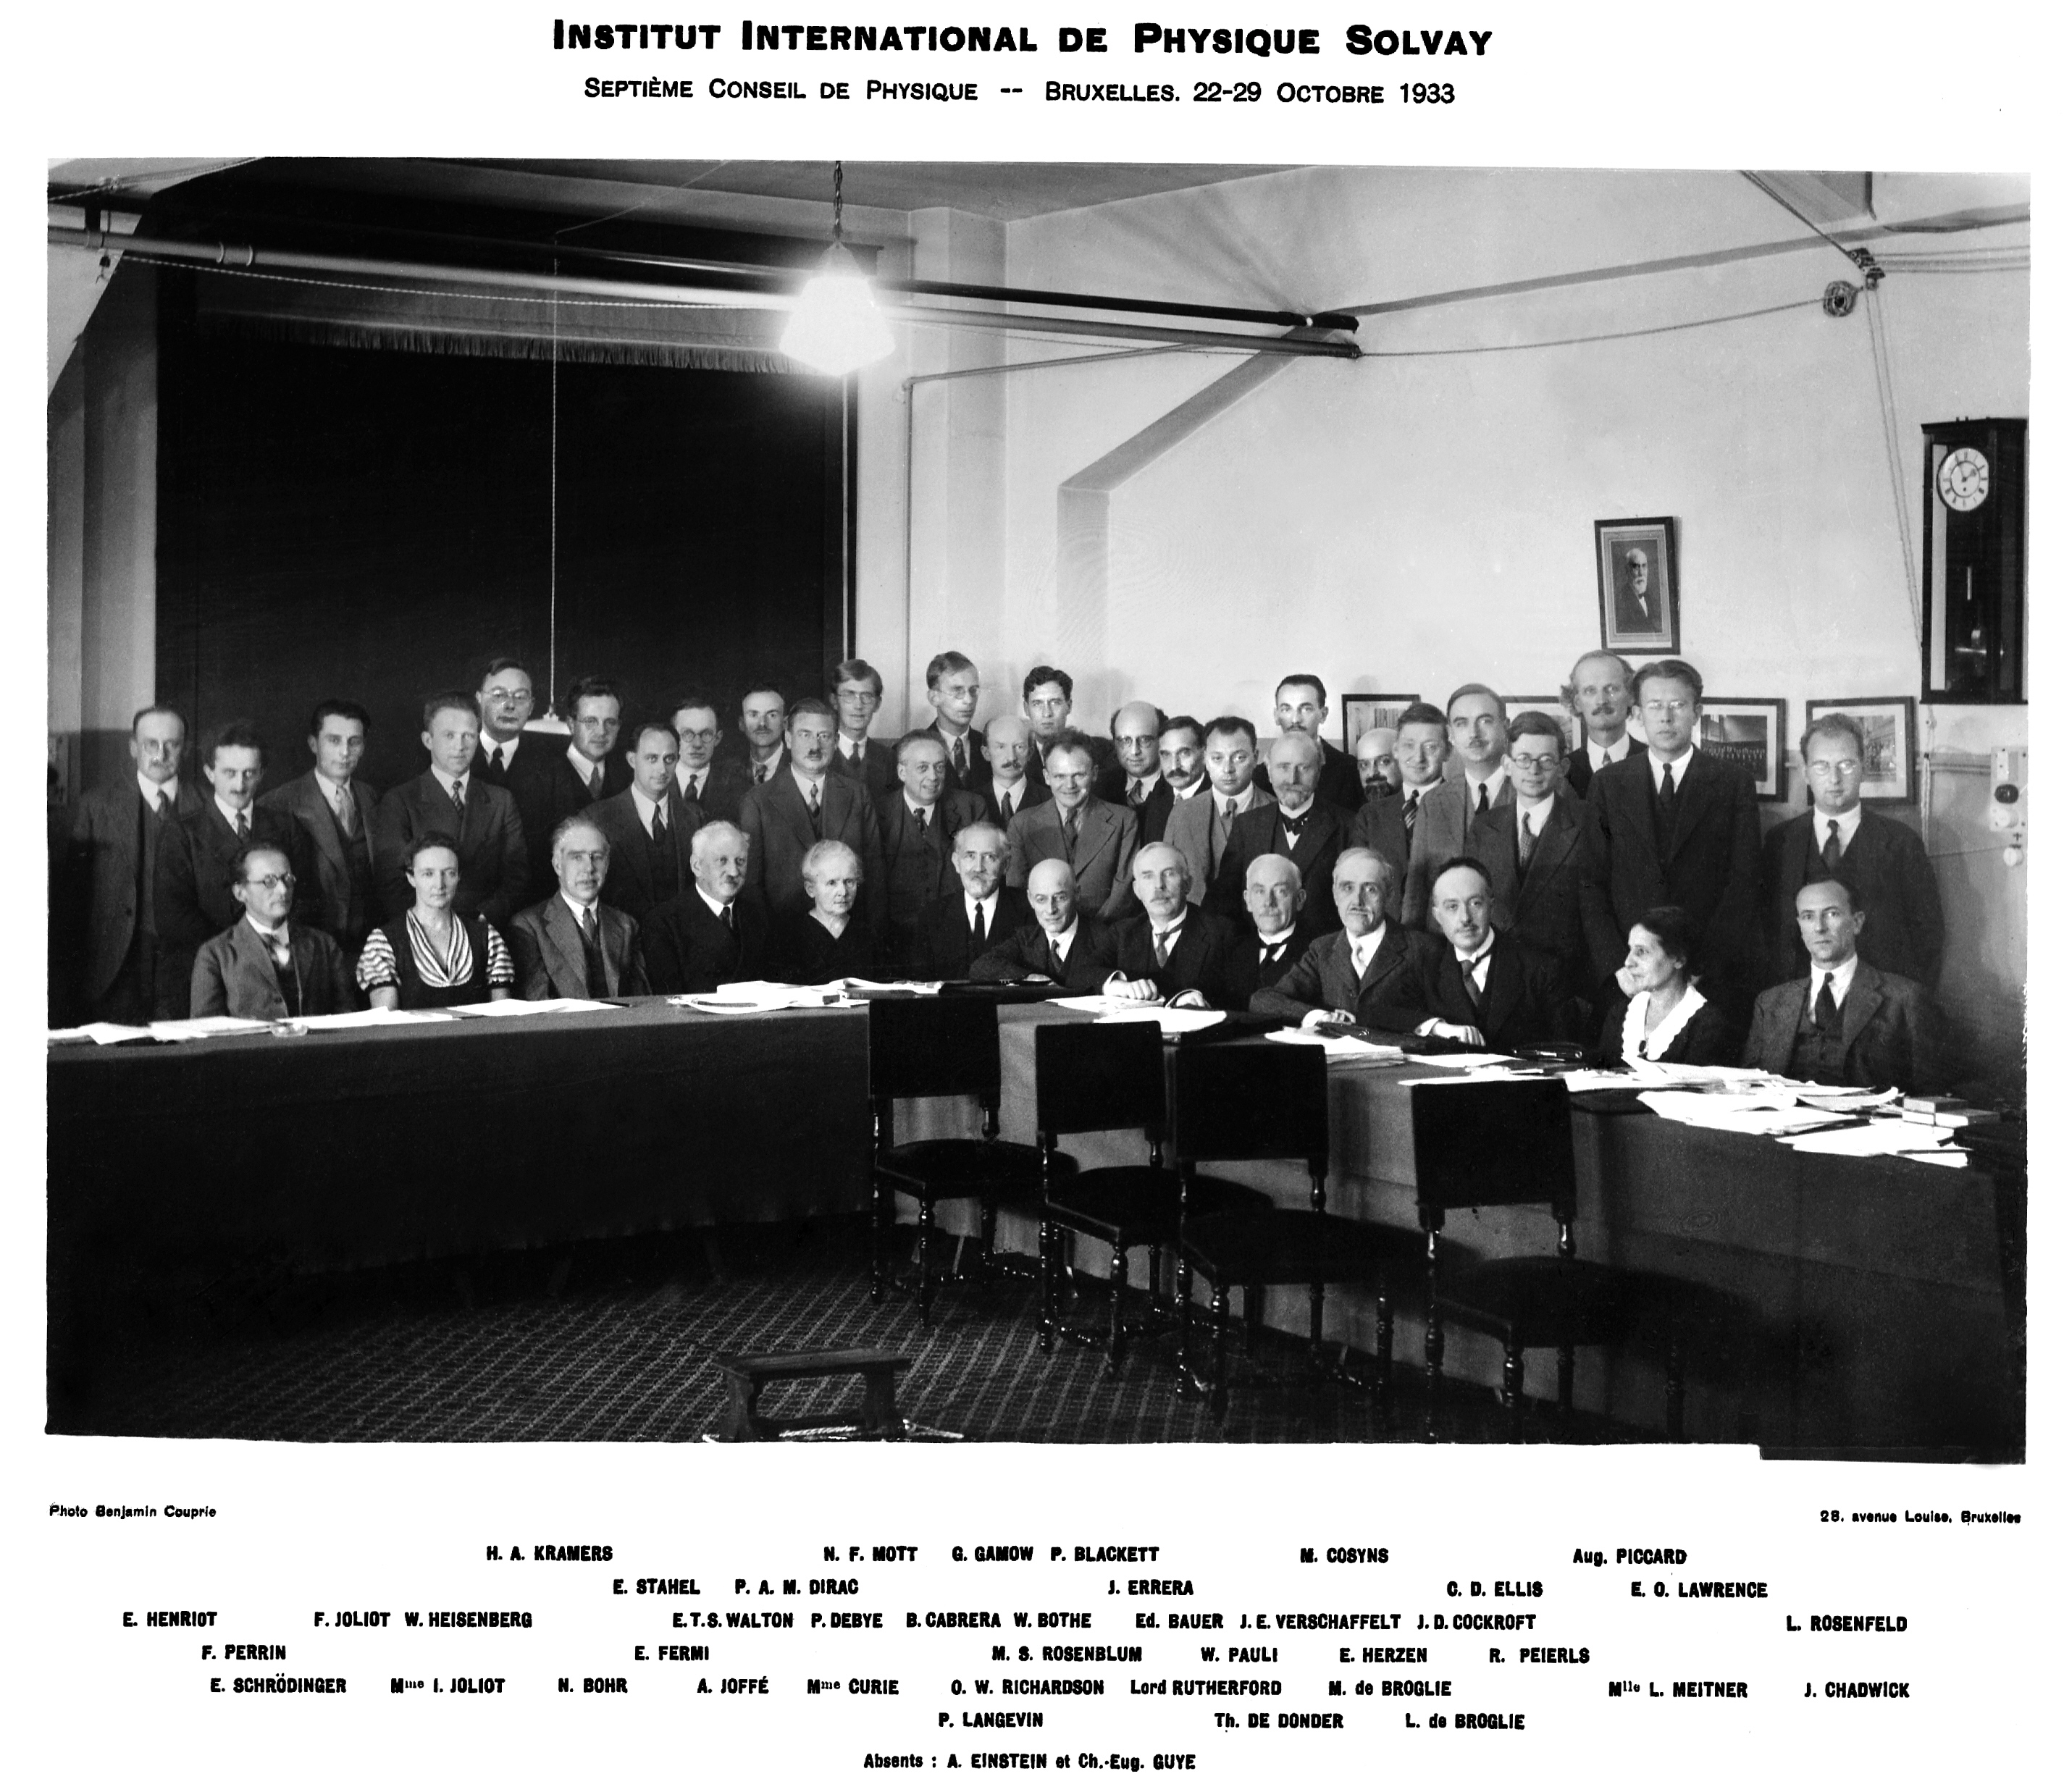
\includegraphics[scale=0.18]{Solvay1933Large.jpg}
% 
% \column{0.6\textwidth}
%%\begin{block}{}
%Pauli in  1933 at the Solvay Congress: ``Regarding the properties of these neutral particles, the atomic weights
%of the radioactive elements tell us first of all that their mass cannot exceed
%much that of the electron. In order to distinguish them from the heavy
%neutrons, Mr. Fermi proposed the name ``neutrino.'' {\bf It's possible that the
%neutrinos' own mass might be equal to zero, so that they would have to
%propagate with the speed of light, like the photons}. However, their penetrating power would exceed by far that of photons of the same energy. It
%seems to me acceptable that the neutrinos have spin 1/2 and satisfy Fermi's 
%statistics, although experiments do not give us any direct proof of this hypothesis. 
%{\bf We know nothing about the interaction of the neutrinos with other material particles and with the photons".}
%
%%\end{block}
%\end{columns}
%\end{frame}
\begin{frame}
\frametitle{What do we talk about when we talk about Dirac?}
\begin{columns}
\column{0.35\textwidth}
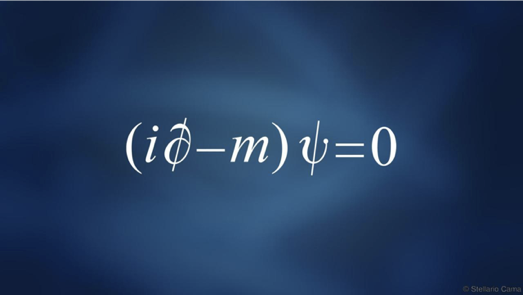
\includegraphics[scale=0.20]{dirac-eq.png}
 
 \column{0.6\textwidth}
%\begin{block}{}
If neutrinos were fermions of spin 1/2 they could presumably described by Dirac equation. Dirac had proposed his famous equation in 1928, two years before the neutrino was proposed by Pauli.  In 1929 P.A.M. Dirac had published his famous paper predicting antimatter (the positron), who would be discovered shortly after by Andersen. Yet, in 1930, antimatter was a concept as fantastic and hard to believe in as the neutrino itself.  

%\end{block}
\end{columns}
\end{frame}

\begin{frame}
\frametitle{The quantum theory of the electron}

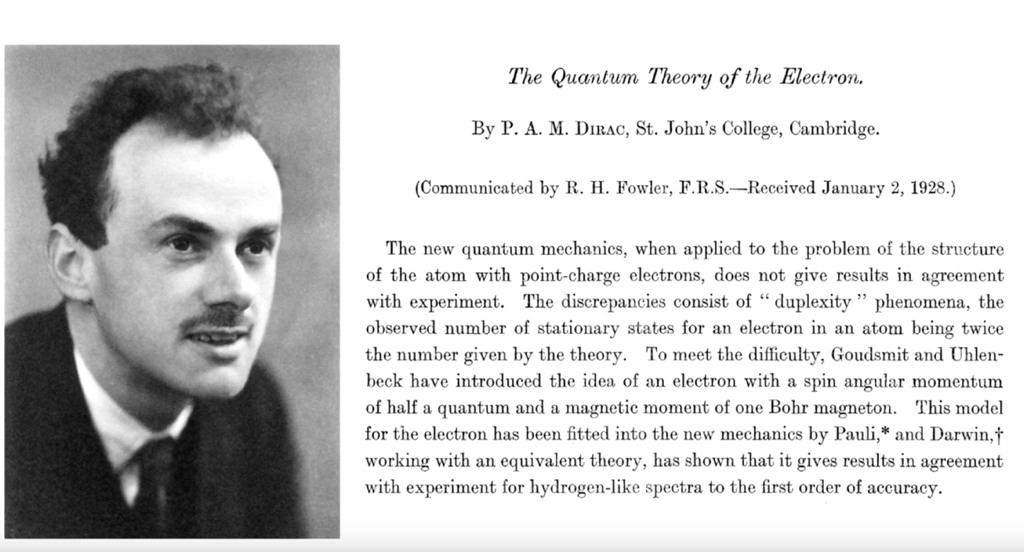
\includegraphics[scale=0.3]{dirac-eq-paper.png}
 
\end{frame}

\begin{frame}
\frametitle{The Klein Gordon equation}
The Dirac equation describes spin-1/2 particles such electrons and neutrinos. It emerges from Dirac's attempt to avoid the negative solutions in the equation of Klein-Gordon which is obtained when one quantizes the relativistic relation:
\[
E^2 = p^2 + m^2 \, \, {(\rm with~ c = 1)}
\]
through the quantum-mechanical recipe:
\[
E \rightarrow i \frac{\partial}{\partial_t}, \,\, \vv{\bm{P}} \rightarrow -i \vv{\bm{\nabla}}
\]
then we obtain the Klein Gordon equation


\begin{empheq}[box=\fbox]{align}
   (i \frac{\partial}{\partial_t})^2 \psi= [(-i \bar{\nabla})^2 + m^2] \psi \nonumber
\end{empheq}

%\[
%(i \frac{\partial}{\partial_t})^2 \psi= [(-i \bar{\nabla})^2 + m^2] \psi
%\]
%which is the KG equation. 

The wavefunction $\psi$~ is now a relativistic scalar and the space and time derivatives are both
second order. However, the initial values of $\psi$~  and
$\partial \psi$~  can be chosen freely, and as a result the probability density is no longer positive definite. 
This leaves open the possibility of negative probabilities.
\end{frame}

%%
\begin{frame}
\frametitle{Plane wave solutions of the KG equation}
If we apply the KG equation to a plane wave
\[
 \psi = A \cdot e^{-ip \cdot x} = A \cdot e^{-i (E\cdot t - p_x \cdot x - p_y \cdot y - p_z \cdot z )}
 \]
 \begin{eqnarray*}
i \frac{\partial}{\partial_t} \psi & = & -i E \psi \\
(i \frac{\partial}{\partial_t})^2 \psi & = & E^2 \psi \\
(-i \vv{\bm{\nabla}})^2 \psi &= &(\frac{\partial}{\partial_x} p_x \cdot x, \frac{\partial}{\partial_y} p_y \cdot y,\frac{\partial}{\partial_z} p_z \cdot z) 
\cdot (\frac{\partial}{\partial_x} p_x \cdot x, \frac{\partial}{\partial_y} p_y \cdot y,\frac{\partial}{\partial_z} p_z \cdot z) \\
&=& (p_x, p_y, p_z) \cdot (p_x, p_y, p_z) = p^2
\end{eqnarray*}
and so we recover $E^2 = p^2 + m^2$.

\vspace{0.5cm}

Since $E = \pm \sqrt{p^2 + m^2}$~negative solutions appear unavoidable. To dodge them, Dirac set to 
construct a wave equation which is linear in the time derivative, hoping that it would yield solutions with only positive energies and positive probabilities.

\end{frame}

\begin{frame}
\frametitle{Linearizing $E = \sqrt{p^2 + m^2}$}
Dirac approach was to attempt linearizing the relativistic energy-momentum equation
\[
E = \sqrt{p^2 + m^2} = \vv{\bm{\alpha}}\cdot \vv{\bm{P}} + \beta \cdot m = 
\alpha_x p_x + \alpha_y p_y + \alpha_z p_z + \beta m
\]
Squaring both sides:

\begin{align*}
E^2 = p^2 + m^2 = & (\alpha_x p_x + \alpha_y p_y + \alpha_z p_z + \beta m) 
(\alpha_x p_x + \alpha_y p_y + \alpha_z p_z + \beta m) \\
%= & \alpha_x^2 p_x^2 + \alpha_y^2 p_y^2 + \alpha_z^2 p_z^2 + \beta^2 m^2 \\
%+ & (\alpha_x \alpha_y + \alpha_y \alpha_x) p_x p_y \\
%+ & (\alpha_x \alpha_z + \alpha_z \alpha_x) p_x p_z \\
%+ & (\alpha_y \alpha_z + \alpha_y \alpha_y) p_y p_z \\
%+ & (\alpha_x \beta + \beta \alpha_x) m p_x \\
%+ & (\alpha_y \beta + \beta \alpha_y) m p_y \\
%+ & (\alpha_z \beta + \beta \alpha_z) m p_z \\
= & p_x^2 + p_y^2 + p_z^2 + m^2
%
\end{align*}
The above equation can only be solved if the $\alpha_i, \beta$~are matrices of at least rank 4, which satisfy:
 \begin{empheq}[box=\fbox]{align}
  \{\alpha_i, \alpha_j\}&=0 \, \, ( i \neq j)\\ 
\{\alpha_i, \beta\} & = 0 \nonumber
\end{empheq}
where:
\[
\{A, B\} = AB + BA
\]
\end{frame}

%%\begin{frame}
\frametitle{Properties of $\bf{\alpha}$~and $\bf{\beta}$ }
\[
\alpha_x^2 p_x^2 + \alpha_y^2 p_y^2 + \alpha_z^2 p_z^2 + \beta^2 m^2 = p_x^2 + p_y^2 + p_z^2 + m^2
\]
Implies

%\begin{empheq}[box=\tcbhighmath]{align}
%a&=b\\
%E&=mc^2 + \int_a^a x\, dx
%\end{empheq}

\begin{empheq}[box=\tcbhighmath]{align}
\alpha_x^2 = \alpha_y^2 = \alpha_z^2 = \beta^2 = 1
\end{empheq}

%\end{block}

Define the anticommutator symbol as:
\[
\{A, B\} = AB + BA
\]

Then
\begin{align*}
& (\alpha_x \alpha_y + \alpha_y \alpha_x) p_x p_y 
+ (\alpha_x \alpha_z + \alpha_z \alpha_x) p_x p_z \\
+ & (\alpha_y \alpha_z + \alpha_y \alpha_y) p_y p_z 
+ (\alpha_x \beta + \beta \alpha_x) m p_x \\
+ & (\alpha_y \beta + \beta \alpha_y) m p_y 
+  (\alpha_z \beta + \beta \alpha_z) m p_z 
= 0
\end{align*}
Implies

\begin{empheq}[box=\tcbhighmath]{align}
\{\alpha_i, \alpha_j\}&=0 \, \, ( i \neq j)\\
\{\alpha_i, \beta\} & = 0
\end{empheq}

%\begin{align*}
%\{\alpha_i, \alpha_j\} = & 0 \, \, ( i \neq j) \\
%\{\alpha_i, \beta\} = & 0 
%
%\end{align*}

\end{frame}

\begin{frame}
\frametitle{Constructing $\bf{\alpha}$~and $\bf{\beta}$~using Pauli matrices }
%\begin{block}{}
%Since the $\alpha, \beta$~do not commute, they cannot be numbers. \alert{They need to be matrices}. In fact, they are traceless hermitian ($A^\dagger = A$) matrices or rank greater or equal than four. 
%\end{block}

They $\alpha, \beta$ can be constructed in terms of the  Pauli matrices:
\[
\alpha_i = 
\begin{pmatrix} 
0 & \sigma_i \\
\sigma_i & 0 
\end{pmatrix} \, \, ,
\beta = 
\begin{pmatrix} 
I & 0 \\
0 & -I 
\end{pmatrix} 
\]

where $I$~is the $2 \times 2$~ identity matrix, and the Pauli matrices are:
\[
\sigma_1 = 
\begin{pmatrix} 
0 & 1 \\
1& 0 
\end{pmatrix} \, \, ,
\sigma_2 = 
\begin{pmatrix} 
0 & -i \\
i & 0 \\ 
\end{pmatrix} \, \, ,
\sigma_3 = 
\begin{pmatrix} 
1 & 0 \\
0 & -1 \\ 
\end{pmatrix}
\]

Pauli matrices exhibit clearly the properties of being hermitian and traceless,
$\sigma_i^\dagger = \sigma_i$, $Tr \sigma_i = 0$, and $\sigma_i^2 = I$. They satisfy the commutation relations: 
\begin{empheq}[box=\fbox]{align}
 %\begin{empheq}[box=\tcbhighmath]{align}
\{\sigma_i, \sigma_j\}&=2 \delta_{ij} \, \, ( i,j,k = 1, 2, 3)\\
[\sigma_i, \sigma_j] & = 2 i \epsilon_{ijk} \sigma_k \nonumber
\end{empheq}
\end{frame}

\begin{frame}
\frametitle{The Dirac equation }
using the linearized equation
\[
E  -\va{\alpha}\cdot \va{P} - \beta \cdot m = 0
\]
and substituting operators
\[
E \rightarrow i \frac{\partial}{\partial_t}, \,\, \va{P} \rightarrow -i \va{\nabla}
\]
One obtains the Dirac equation
\[
 i \frac{\partial}{\partial_t} \psi = [ \va{\alpha} (-i\va{\nabla}) + m] \psi
\]

Multiply now $\beta$~from the left and define  the gamma matrices:
\[
 \gamma^0 = \beta = \begin{pmatrix} 
I & 0 \\
0 & -I 
\end{pmatrix}  \,\,\, ,  \gamma^i = \beta \alpha_i = \begin{pmatrix} 
0 & \sigma_i \\
-\sigma_i & 0 
\end{pmatrix} 
\]
To obtain 
%
%\begin{empheq}[box=\fbox]{align}
%(E \gamma^0 -\va{p}\cdot \va{\gamma} -m ) \psi & = 0 \nonumber
%\end{empheq}
%\[
%[i(\gamma^0 \partial_0 + \gamma^i \partial_i) -m ] \psi  = 0
%\]
%or
 \begin{empheq}[box=\fbox]{align}
(i \gamma^\mu \partial_\mu -m ) \psi & = 0 \nonumber
\end{empheq}
\end{frame}

%\begin{frame}
%Alternatively, in terms of the energy and momentum operators:
%\begin{empheq}[box=\fbox]{align}
%(E \gamma^0 -\va{p}\cdot \va{\gamma} -m ) \psi & = 0 \nonumber
%\end{empheq}
%
%In this equation $\psi$~is the Dirac bispinor: 
%\[
%\psi = \mqty(\psi_1 \\ \psi_2 \\ \psi_3 \\ \psi_4) =  \mqty(\phi \\ \chi); \,\,\,
%\phi =  \mqty(\phi_1 \\ \phi_2), \,\,\, \chi =  \mqty(\chi_1 \\ \chi_2)
%\]
%The two spinors $\phi$~and $\chi$~represent the particle and the antiparticle; the two components of each of them represent the two states of the third component of the spin, $s_z = +1/2$~and
%$s_z = -1/2$.
%
%The four $\gamma$~matrices, found before, are not unique. Any set that satisfy the anticommutation relations (Clifford algebra) can be used:
%
%\begin{empheq}[box=\fbox]{align}
%\{\gamma^\mu, \gamma^\nu\} = 2 g^{\mu\nu} \nonumber
%\end{empheq}
%\end{frame}

%%\begin{frame}
\frametitle{The Dirac equation }
The Dirac equation can also be written as: 

 \begin{empheq}[box=\tcbhighmath]{align}
(E \gamma^0 -\va{p}\cdot \va{\gamma} -m ) \psi & = 0
\end{empheq}

In this equation $\psi$~is the Dirac bispinor: 
\[
\psi = \mqty(\psi_1 \\ \psi_2 \\ \psi_3 \\ \psi_4) =  \mqty(\phi \\ \chi); \,\,\,
\phi =  \mqty(\phi_1 \\ \phi_2), \,\,\, \chi =  \mqty(\chi_1 \\ \chi_2)
\]
The two spinors $\phi$~and $\chi$~represent the particle and the antiparticle; the two components of each of them represent the two states of the third component of the spin, $s_z = +1/2$~and
$s_z = -1/2$.

The four $\gamma$~matrices, found before, are not unique. Any set that satisfy the anticommutation relations (Clifford algebra) can be used:

 \begin{empheq}[box=\tcbhighmath]{align}
\{\gamma^\mu, \gamma^\nu\} = 2 g^{\mu\nu}
\end{empheq}

\end{frame}

%\begin{frame}
%\frametitle{The Dirac representation of the $\gamma$~matrices} 
%
%\[
%\gamma^0 = \mqty(I & 0 \\ 0 & -I), \,\,\,  \gamma^i = \mqty(0 & \sigma_i \\ -\sigma_i & 0)
%\]
%where the elements are $2 \times 2$~matrices and the $\sigma$~are the Pauli matrices:
%\[
%\sigma^1 = \mqty(0 & 1 \\ 1 & 0), \,\,\,  \sigma^2 = \mqty(0 & -i \\ -i & 0), \,\,\,
%\sigma^3 = \mqty(1 & 0 \\ 0 & -1)
%\]
%To be explicit we can write the full expansion of the Dirac equation:
%\[
%\begin{split}
% i \left[
%\left( \begin{array}{cccc}
%1 & 0 & 0 &0 \\
%0 & 1 & 0 &0 \\
%0 & 0 & -1 &0 \\
%0 & 0 & 0 & -1 \\
%\end{array} \right ) \partial_0 +  
%\left( \begin{array}{cccc}
%0 & 0 & 0 &1 \\
%0 & 0 & 1 &0 \\
%0 & -1 & 0 &0 \\
%-1 & 0 & 0 &0 \\
%\end{array} \right ) \partial_1 + 
% \left( \begin{array}{cccc}
%0 & 0 & 0 &-i \\
%0 & 0 &  i &0 \\
%0 & i & 0 &0 \\
%-i & 0 & 0 &0 \\
%\end{array} \right ) \partial_2   +  \right. \\
%\left. \left( \begin{array}{cccc}
%0 & 0 & 1 &0 \\
%0 & 0 & 0 &-1 \\
%-1 & 0 & 0 &0 \\
%0 & 1 & 0 &0 \\
%\end{array} \right ) \partial_3 
%\right] \left( \begin{array}{c}
%\psi_1 \\
%\psi_2 \\
%\psi_3 \\
%\psi_4 \\
%\end{array} \right )  = m \left( \begin{array}{c}
%\psi_1 \\
%\psi_2 \\
%\psi_3 \\
%\psi_4 \\
%\end{array} \right )
%\end{split}
%\]
%\end{frame}

%%\begin{frame}
\frametitle{The explicit Dirac equation: alternatives to the $\gamma$~matrices}

\[
\begin{split}
 i \left[
\left( \begin{array}{cccc}
1 & 0 & 0 &0 \\
1 & 0 & 0 &0 \\
1 & 0 & 0 &0 \\
1 & 0 & 0 &0 \\
\end{array} \right ) \partial_0 +  
\left( \begin{array}{cccc}
1 & 0 & 0 &0 \\
1 & 0 & 0 &0 \\
1 & 0 & 0 &0 \\
1 & 0 & 0 &0 \\
\end{array} \right ) \partial_1 + 
 \left( \begin{array}{cccc}
1 & 0 & 0 &0 \\
1 & 0 & 0 &0 \\
1 & 0 & 0 &0 \\
1 & 0 & 0 &0 \\
\end{array} \right ) \partial_2   +  \right. \\
\left. \left( \begin{array}{cccc}
1 & 0 & 0 &0 \\
1 & 0 & 0 &0 \\
1 & 0 & 0 &0 \\
1 & 0 & 0 &0 \\
\end{array} \right ) \partial_3 
\right] \left( \begin{array}{c}
\psi_1 \\
\psi_2 \\
\psi_3 \\
\psi_4 \\
\end{array} \right )  = m \left( \begin{array}{c}
\psi_1 \\
\psi_2 \\
\psi_3 \\
\psi_4 \\
\end{array} \right )
\end{split}
\]
%\begin{alertblock}{Important theorem}
Searching for a linear equation, Dirac found a system of 4 equations, operating over a 4-dimensional waveform. Notice, however, that the $\gamma$~matrices are not the only explicit expression that satisfies the Clifford algebra $\{\gamma^\mu, \gamma^\nu\} = 2 g^{\mu\nu}$. There are other possible representations, such as the Weyl, and the Majorana representation. The former is specially well suited to describe massless neutrinos. The later was used by Majorana to propose the hypothesis that the neutrino could be its own antiparticle. 
%\end{alertblock}
\end{frame}

%%\begin{frame}
\frametitle{The classical view of Spin}
\begin{columns}
 
\column{0.5\textwidth}
\includegraphics[scale=0.1]{electronMagnet.png}
The cartoon pictures the ``classical'' view of an atom (hydrogen), seen as a tiny magnet. The electron ``orbiting'' around the nucleus is said to have an (orbital) angular momentum defined by:
\[
\vv{\bm{L}} = \vv{\bm{r}} \times \vv{\bm{p}} 
\]

From a classical perspective, as an electron carries a charge, its orbital motion will result in a tiny current loop which will produce a dipolar magnetic field. The strength of this dipole field is measured by the magnetic moment $\mu$ which is related to the orbital angular momentum by:
\[
\vv{\bm{\mu_L}} = \frac{q}{2m}\vv{\bm{L}} 
\]
\column{0.5\textwidth}
\includegraphics[scale=0.1]{classicalElectronSpin.png}
The classical idea of spin follows directly from the above considerations. Spin is the angular momentum we associate with a rotating sphere. If the sphere possesses an electric charge, then the circulation of the charge around the axis of rotation will constitute a current and hence will give rise to a magnetic field. This field is a dipole field whose strength, for a uniformly charged sphere of total charge q, is:

\[
\vv{\bm{\mu_L}} = \frac{q}{2m}\vv{\bm{S}} 
\]
\end{columns}



\end{frame}
%%\begin{frame}
\frametitle{Spin is a quantum effect}
 
The classical view of spin requires that the spinning sphere example has a non-zero radius. Classically a point particle can only have a spin angular momentum of zero and so it cannot have a magnetic moment. Thus, from the point-of-view of classical physics, elementary particles such as an electron, which are known to possess spin angular momentum, cannot be viewed as point objects -- they must be considered as tiny spinning spheres. But high energy scattering experiments show that \alert{elementary particles such as the electron behave very much as point particles}, with a radius smaller than $10^{-17}$~m. Yet they are found to possess magnetic moment and thus spin angular momentum of a magnitude equal (for the electron) to 
$\frac{\sqrt{3}}{2} \hbar$which requires the surface of the particle to be moving at a speed greater than that of light. 
 
\begin{alertblock}{The electron spin is a purely quantum effect}
The classical picture of an elementary particle as a tiny, rapidly rotating sphere is untenable.
\end{alertblock}
 \end{frame}

%%\begin{frame}
\frametitle{Quantum angular momentum and space quantization}
 
Quantum wave mechanics provides, via the quantum mechanical version of 
$\vv{\bm{L}} = \vv{\bm{r}} \times \vv{\bm{p}}$
a quantum description of the orbital angular momentum of a particle, such as that associated with an electron moving in an orbit around an atomic nucleus. The general results found are that the magnitude of the angular momentum is limited to the values:
\[
L = \sqrt{l(l+1)}\hbar, \, \, \, l = 0,1,2,3
\]

The quantum theory of orbital angular momentum also states that any one vector component of 
$\vv{\bm{L}}$, say $L_z$~Lz  is restricted to the values:
\[
L = m_l\hbar, \, \, \, m_l = -l, -l+1, -l+2....l-1, l.
\]

This restriction on the possible values of $L_z$~ mean that the angular momentum vector can have only
certain orientations in space --a result known as ``space quantization''.

All this is built around the quantum mechanical version of $\vv{\bm{L}} = \vv{\bm{r}} \times \vv{\bm{p}}$, and so implicitly is concerned with the angular momentum of a particle moving through space. In this sense the quantization of angular momentum is a necessary consequence of wave mechanics. \alert{However, the quantization of $\vv{\bm{L}}$, does not explain or predict the existence of an intrinsic angular momentum
$\vv{\bm{S}}$}.
\end{frame}

%%\begin{frame}
\frametitle{The Stern Gerlach experiment: an attempt to test space quantization}
\begin{columns}
 
\column{0.5\textwidth}
\includegraphics[scale=0.2]{sternGerlach3.png}
In the Stern-Gerlach experiment (1922) a beam of silver atoms passed through an inhomogeneous magnetic field as shown in the sketch. The experiment was intended to test the space-quantization associated with the orbital angular momentum of atomic electrons, already described by the ``old quantum theory'' (Sommerfeld) which could be tested by making use of the fact that an orbiting electron will give rise to a magnetic moment proportional to the orbital angular momentum of the electron. 
\column{0.5\textwidth}
\includegraphics[scale=0.2]{sgSpots.jpg}
The result of the experiment is shown  (picture from the original paper). There is an intensity minimum in the center of the pattern, and the separation of the beam into two components is clearly seen. This result seemed to confirm Sommerfeld's quantum-theoretical prediction of spatial quantization. 
%Pauli, a notoriously skeptical physicist, remarked, ``Hopefully now even the incredulous Stern will be convinced about directional quantization'' (in a letter from Pauli to Gerlach 17 February 1922). 
\end{columns}



\end{frame}
%%\begin{frame}
\frametitle{Stern Gerlach experiment: Spin is real}

There are 47 electrons surrounding the silver atom nucleus, of which 46 form a closed inner core of total angular momentum zero -- there is no orbital angular momentum, and the electrons with opposite spins pair off, so the total angular momentum is zero, and hence there is no magnetic moment due to the core. The one remaining electron also has zero orbital angular momentum, \alert{so the sole source of any magnetic moment is that due to the intrinsic spin of the electron.}
 
Thus, the experiment represents a direct measurement of one component of the spin of the electron, this component being determined by the direction of the magnetic field, here taken to be in the z direction.

There are two possible values for $S_z$~ corresponding to the two spots on the observation screen, implying that $s = 1/2$. The allowed values for the $z$~component of the spin are:
\[
S_z = \pm \frac{1}{2}\hbar
\]

Of course there is nothing special about the direction $z$. Any component of the spin of an electron will have only two values. If $\vv{\bm{n}}$ is a unit vector specifying some arbitrary direction then:
\[
\vv{\bm{S}} \cdot \vv{\bm{n}} = \pm \frac{1}{2}\hbar
\]
\end{frame}
%%\begin{frame}
\frametitle{What do we talk about when we talk about spin? NRQM and Pauli matrices}

In NRQM we define $\ket{\uparrow}$~to be the state with spin in the $+z$~direction and 
$\ket{\downarrow}$~to be the state with spin in the $-z$~direction.
 
\[
\ket{\uparrow} = \mqty(1\\0), \,\,\, \ket{\downarrow} = \mqty(0\\1)
\]

In the space spanned by $\ket{\uparrow}$~and $\ket{\downarrow}$~the angular momentum operator is represented by the Pauli matrices
\[
J_i =\frac{\sigma_i}{2}, \,\,\, (i=1,2,3, ~{\rm or}~x,y,z)
\]
which satisfy the commutation relation of angular momentum operators, 
$[J_i, J_k] = i \epsilon_{ijk} J_k$. The square of the angular momentum operator $\va{J^2}$ is:
\[
\va{J^2} =J_1^2 + J_2^2 + J_2^2 = j(j+1)
\]
But then: 
\[
\frac{\va{\sigma^2}}{2} =(\frac{\sigma_1}{2})^2 + (\frac{\sigma_2}{2})^2 + (\frac{\sigma_3}{2})^2 
= \frac{3}{4} = \frac{1}{2}(\frac{1}{2} + 1)
\]
$\va{\sigma}/2$~ is  a spin-1/2 representation of angular momentum.
\end{frame}
%%\begin{frame}
\frametitle{What do we talk about when we talk about spin? Spin along an arbitrary direction}


The eigenstates with spin polarized along an arbitrary unit vector $\va{s}$~ 
can be obtained by applying a rotation to the states $\ket{\uparrow}$~ and $\ket{\downarrow}$.

 The rotation operator $R(\va{\theta})$~by an angle $\theta = \abs{\va{\theta}}$~
 around the axis $\hat{\theta} = \va{\theta}/\theta$~is generated by the angular momentum operators
 \[
 R(\va{\theta}) = e^{-i \va{\theta}\cdot \va{J}}
 \]
 In the spin 1/2 space, the corresponding rotation $u(\va{\theta})$~is a $2 \times 2$~matrix obtained
 by replacement $\va{J} \rightarrow \va{\sigma}/2$.
 \[
 u(\va{\theta}) = e^{-i \frac{\va{\theta}}{2}\va{\sigma}} = \cos{\frac{\theta}{2}} - i (\hat{\theta} \cdot \va{\sigma)}\sin{\frac{\theta}{2}}
 \]

\end{frame}
%%\begin{frame}
\frametitle{Rotation matrix}

\includegraphics[scale=0.7]{rotation.png}
The z-axis can be rotated to the direction of $\va{s}$~  by first rotating around the y-axis by $\theta$~ and then around the original z-axis (not the rotated one) by $\phi$~, where $(\theta,\phi)$~ are the polar angles of the direction $\va{s}$. 
 \[
 \va{s} = (s_x, s_y, s_z) = (\sin\theta\cos\phi, \sin\theta\sin\phi, \cos\theta).
 \]

The rotation matrix is then: 
 \[
 R(\theta, \phi) = e^{-i\frac{\phi}{2}\sigma_z} e^{-i\frac{\theta}{2}\sigma_y}
 \]

 \end{frame}
 
 \begin{frame}
\frametitle{Eigenvectors of spin in an arbitrary direction}

 \begin{eqnarray*}
 \chi_{+} &= & u(\theta, \phi) \mqty(1\\0) = \frac{1}{\sqrt{2(1 + s_z)}}\mqty(1 + s_z\\ s_{+})\\
\chi_{-} &= & u(\theta, \phi) \mqty(0\\1) = \frac{1}{\sqrt{2(1 - s_z)}}\mqty( s_z - 1\\ s_{-})\\
\end{eqnarray*}
where
\[
s_{\pm} = s_x \pm i s_y
\]
The spin component in an arbitrary direction $\va{s}$~ is represented by the operator
$\va{s} \cdot \va{\sigma}$~(in units of the absolute value of the spin, which is 1/2)
 
 \begin{eqnarray*}
\va{s} \cdot \va{\sigma} &= &s_x \mqty(0 & 1\\ 1 & 0) + s_y \mqty(0 & -i\\ i & 0) + s_z \mqty(1 & 0\\ 0 & -1) \\
& = &  \mqty(s_z & s_x - i s_y\\ s_x + i s_y & -s_z) =
  \mqty(s_z & s_{-}\\ s_{+} &  -s_z) 
\end{eqnarray*}
 \end{frame}
 
 
  \begin{frame}
\frametitle{Projection operators}

Using the fact that $\va{s} \cdot \va{\sigma}$~has eigenvalues $\pm 1$, we can construct
projection operators which project out $\chi_{\pm}$ from any vector:

\[
P_{\pm} = \frac{1 \pm \va{s} \cdot \va{\sigma}}{2}
\]
Writing any vector $v$~as a linear combination of $\chi_{\pm}$, $v = c_{+}\chi_{+} + c_{-}\chi_{-}$, we can see that $P_{\pm}$~projects out $\chi_{\pm}$~out of $v$
\[
P_{+} v = c_{+} \chi_{+}, \,\,\, P_{-} v = c_{-} \chi_{-}
\]

 \end{frame}
%%\begin{frame}
\frametitle{What do we talk about when we talk about spin? Spin in the Dirac equation}

We can represent rotations in spinor space through the corresponding representation of the Lorentz group: 
 \[
 U(\va{\theta}) = e ^{-i \theta_i\frac{\Sigma_i}{2}}
 \]
where $\Sigma_i$~can be constructed in terms of the Pauli matrices:
 \[
 \Sigma_i = \mqty(\sigma_i & 0\\ 0 & \sigma_i)
 \]
We can now write the Dirac equation in terms of the Hamiltonian: 
\[
i \pdv{t} \psi = H \psi, \,\,\, H = \gamma^0(\gamma^i p^i + m)
\]
%where the $\alpha$~and $\beta$~matrices are related with the $\gamma$~matrices. 
%\[
% \gamma^0 = \beta   \,\,\, ,  \gamma^i = \beta \alpha_i 
% \]
%\end{frame}
Now we can enquire if the angular momentum commutes with H (ergo a constant of motion). 
%Write:
%\begin{eqnarray*}
%L_i &= &(\va{x} \times \va{p})_i = \epsilon_{ijk} x^j p^k \\
%H & = & \alpha_i p^i + \beta m = \gamma^0(\gamma^i p^i + m) 
%\end{eqnarray*}
\end{frame}
\begin{frame}
then we find that: 
%\[
%[L_i, H] = i (\va{\alpha} \times \va{p})_i
%\]
%\[
%[\Sigma_i, H]  =-2i (\va{\alpha} \times \va{p})_i
%\]
\[
[L_i, H]  \ne 0 
\]
\[
[\Sigma_i, H]  \ne 0 
\]
And thus, neither $L$, nor $\Sigma$~are constants of motion. Instead we find that:

\[
[\va{J}, H] = 0, \,\,\, \va{J} = \va{L} + \frac{\va{\Sigma}}{2}
\]

\begin{alertblock}{The Dirac equation describes the spin of the electron}
The angular momentum in the Dirac equation is conserved only when the spin is added to the orbital momentum. 
\end{alertblock} 

\end{frame}

\begin{frame}
\frametitle{Is Spin real?}
\begin{block}{}
\begin{itemize}
\item \alert{Yes}. We need spin to explain Stern-Gerlach. In fact we could define spin as the stuff that results in the Stern-Gerlach experiment behavior.
\item \alert{Yes}. Spin emerges out of the Dirac equation which describes the electron (and the neutrino) as spin 1/2 particle. 
\item Spin is a pure quantum effect without a classical counterpart. The rotating sphere used to pictorially describe it is just a (perhaps confusing) metaphor. 
\end{itemize}
\end{block}
\end{frame}
\begin{frame}
\frametitle{Plane wave solutions of the Dirac equation}
For a particle at rest, $\va{p} = 0$ and the Dirac equation becomes:
\[
i\gamma^0\partial_0\psi = m \psi, \,\,\, or \, \, \,  i \mqty(1 & 0 & 0 & 0\\ 0 & 1 & 0 & 0 \\
0 & 0 & -1 & 0 \\ 0 & 0 & 0 & -1 ) \ \mqty(\dot{\psi_1} \\ \dot{\psi_2}\\ \dot{\psi_3} \\ \dot{\psi_4}) = 
m \mqty(\psi_1 \\ \psi_2\\ \psi_3 \\ \psi_4)
\]
There are four independent solutions: two describe particle-antiparticle and two describe spin up-down
\[
\psi^{(1)} = w^{(1)} e^{-i m\cdot t}, \,\,\, \psi^{(2)} = w^{(2)} e^{-i m\cdot t}, \,\,\,
\psi^{(3)} = w^{(3)} e^{+i m\cdot t}, \,\,\, \psi^{(4)} = w^{(4)} e^{i m\cdot t}
\]
\[
w^{(1)} = \mqty(1 \\ 0 \\ 0 \\ 0), \,\,\, w^{(1)} = \mqty(0\\ 1 \\ 0 \\ 0), \,\,\,
w^{(3)} = \mqty(0 \\ 0 \\ 1 \\ 0), \,\,\, w^{(4)} = \mqty(0 \\ 0 \\ 0 \\ 1), \,\,\,
\]

\end{frame}
%\begin{frame}
%\frametitle{The solutions are eigenvalues of the spin}
%The solutions are eigenvalues of the z-component of the spin, $\Sigma_3$, which in the Dirac representation is:
%\[
%\Sigma_3 = \mqty(\sigma_3 & 0 \\ 0 &  \sigma_3) = \mqty(1 & 0 & 0 & 0\\ 0 & -1 & 0 & 0 \\
%0 & 0 & 1 & 0 \\ 0 & 0 & 0 & -1 )
%\]
%thus:
%\[
%\psi^{(1)} : \Sigma_3 = +1, \,\,\,
%\psi^{(2)} : \Sigma_3 = -1, \,\,\,
%\psi^{(3)} : \Sigma_3 = +1, \,\,\,
%\psi^{(4)} : \Sigma_3 = -1.
%\]
%\end{frame}
%
\begin{frame}
\frametitle{Negative energy solutions}

Since we define the eigenvalue of the operator $\pdv{t}$~to be the energy, we find that 
$\psi^{(1)}$~and $\psi^{(2)}$~are positive energy solutions and 
$\psi^{(3)}$~and $\psi^{(4)}$~are negative energy solutions.

\begin{alertblock}{Surprise!}
Dirac's equation \alert{predicts} negative energy solutions.
\end{alertblock}
\end{frame}

\begin{frame}
\frametitle{Dirac struggle with negative energy solutions: protons}

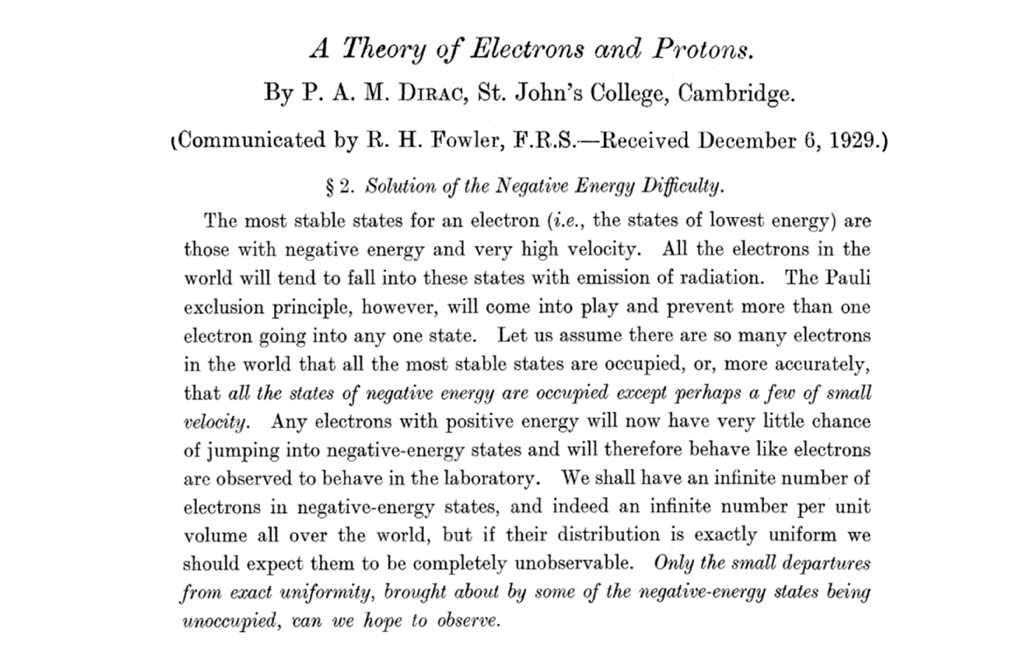
\includegraphics[scale=0.3]{img/DiracElectronProton.png}
\end{frame}

\begin{frame}
\frametitle{The opinion of Heisemberg}

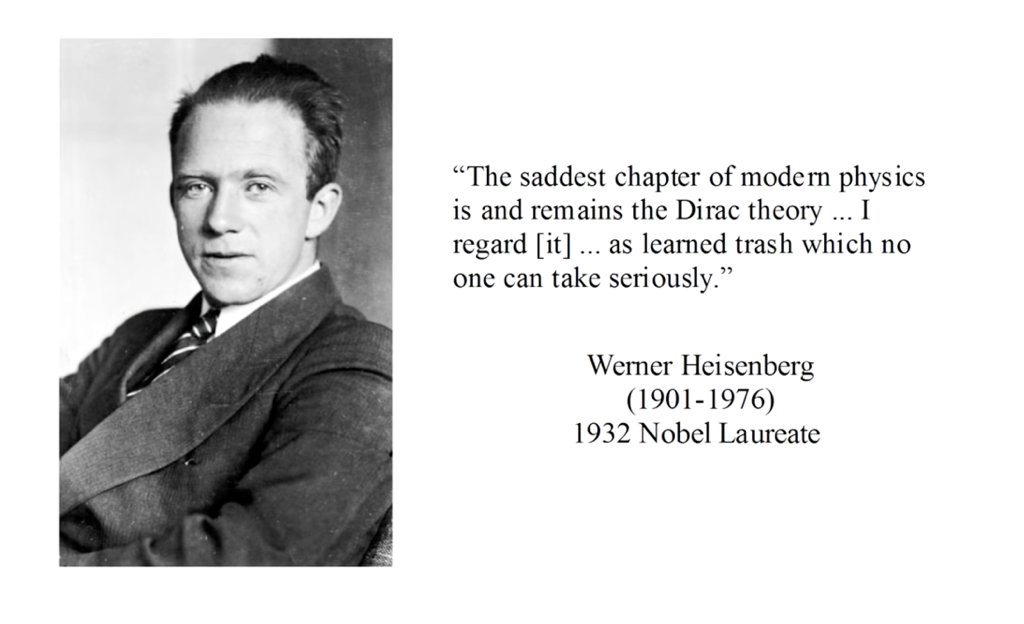
\includegraphics[scale=0.3]{img/HeisembergOpinionDirac.png}
\end{frame}

\begin{frame}
\frametitle{Identifying holes in the negative sea with positrons}

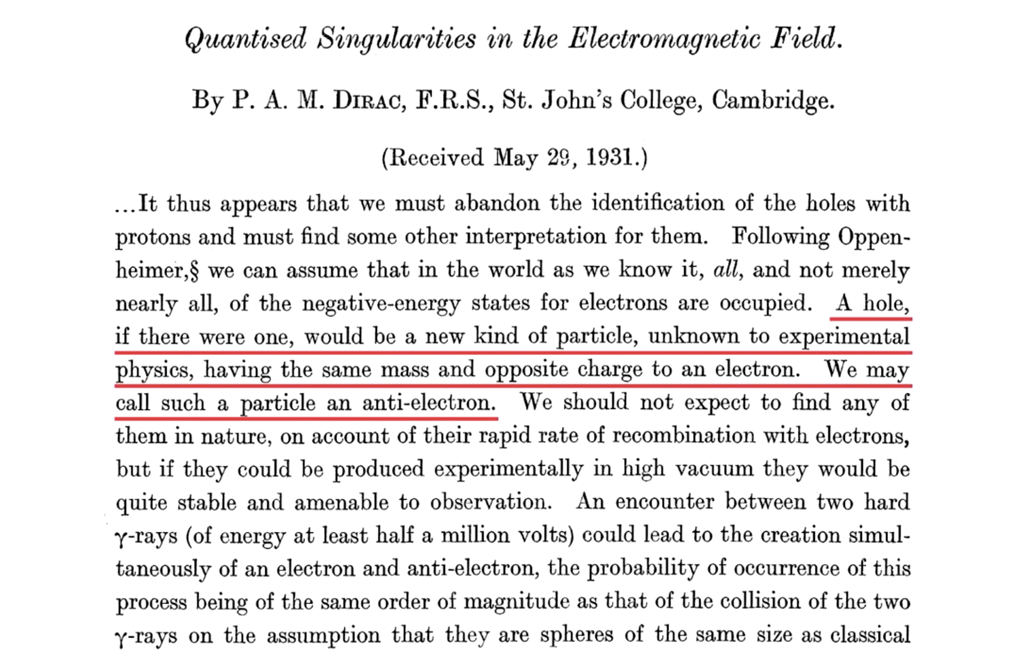
\includegraphics[scale=0.3]{img/diracPositrons.png}
\end{frame}

\begin{frame}
\frametitle{The discovery of the positron (Andersen, 1932)}

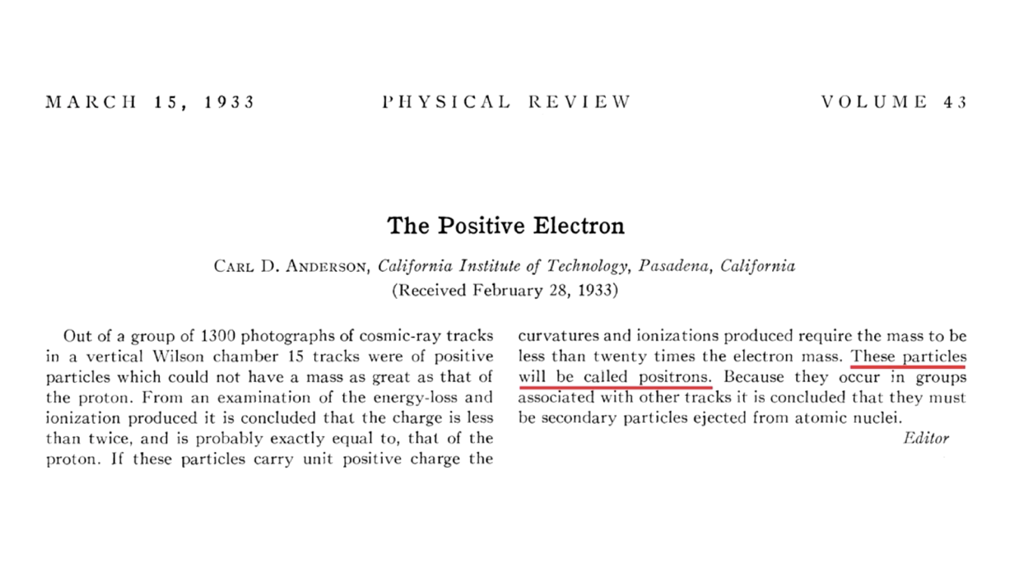
\includegraphics[scale=0.3]{img/AndersonPaper.png}
\end{frame}

%\begin{frame}
%\frametitle{The positron is real}
%
%\includegraphics[scale=0.3]{positronDiscovery.png}
%\end{frame}
%

\begin{frame}
\frametitle{The negative sea parable}

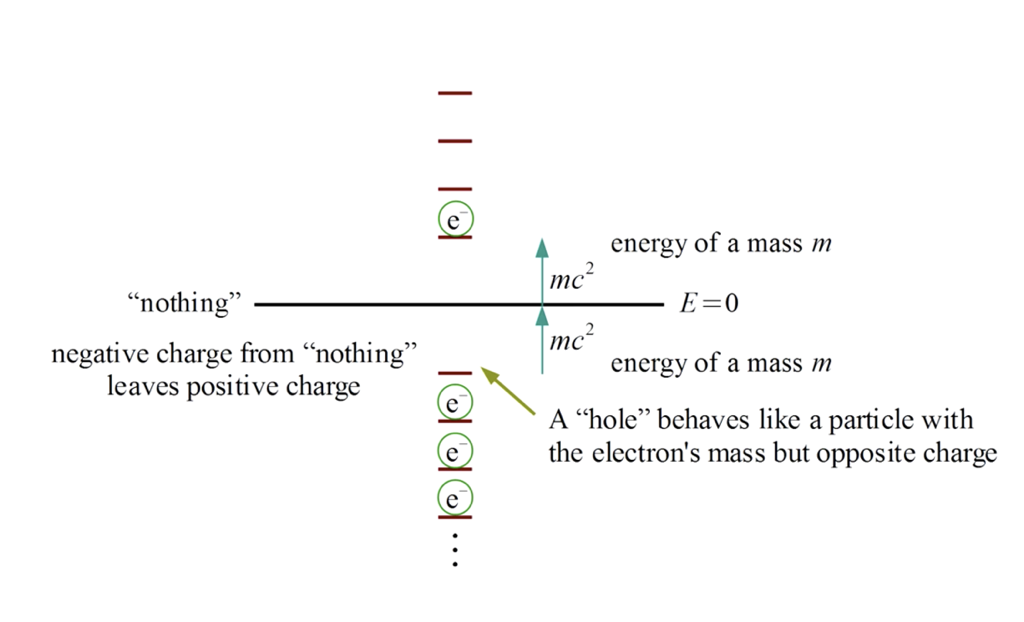
\includegraphics[scale=0.3]{img/negativeSea.png}
\end{frame}

%\begin{frame}
%\frametitle{Relativistic quantum mechanics is not enough}
%
%\includegraphics[scale=0.3]{problemsRQM.png}
%\end{frame}
%
%\begin{frame}
%\frametitle{QFT for pedestrians}
%
%\includegraphics[scale=0.3]{FeymanDiagram.png}
%\end{frame}
%
%\begin{frame}
%\frametitle{QED diagrams}
%
%\includegraphics[scale=0.3]{QEDDiagrams.png}
%\end{frame}







\begin{frame}
\frametitle{The need of Quantum Field Theory}
In spite of the heroic efforts of Dirac and others, RQM is not enough to describe elementary particles. The Dirc equation describes a single electron. Positrons need to be introduced by a sort of magical incantation (the negative sea state). In short, RQM cannot predict creation and annihilation of particles. 

Quantum Electrodynamics (QED) was eventually developed as the first Quantum Field Theory (QFT), capable of describing such creation and annihilation of particles. In QED, it is not only the photons that are quanta of a field but also the charged particles, like the electrons and positrons. The fields are operators that create and annihilate their quanta. \alert{Thus $\psi(x)$~is no longer interpreted as a waveform that describes probability but as an operator that creates a particle in point $x$~and destroys an antiparticle in $x$ ($\bar{\psi}(x)$~will create an antiparticle in point $x$~and destroy antiparticle in $x$)}.

%The Lagrangian of the free Dirac field $\psi$~is given by:
%
%\begin{empheq}[box=\fbox]{align}
%  L = \bar{\psi}(i\gamma^\mu \partial_\mu -m)\psi  \nonumber
%\end{empheq}
%
%where $\bar{\psi} = \psi^\dagger \gamma^0$. Varying the Lagrangian yields back the Dirac equation.

%The $\gamma$~matrices found by Dirac were complex. This means that the spinor field $\psi$~must also be complex. This makes sense from the point of view of field theory as a complex field would create particles and annihilate anti-particles while its complex conjugate would create anti-particles and annihilate particles. However, as we shall see, Majorana found an alternative. 

\end{frame}

\begin{frame}
\frametitle{Feynman Diagrams}
\begin{columns}
\column{0.4\textwidth}
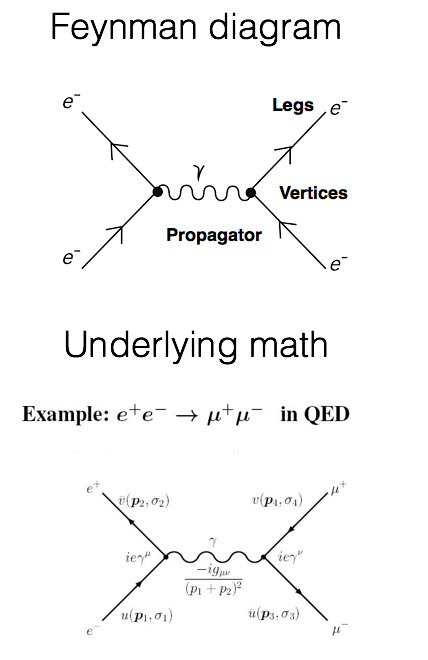
\includegraphics[scale=0.3]{img/FeynmanD2.png}
 
\column{0.5\textwidth}
Feynman diagrams: ``pictures'' whose lines are world-lines of the particles in the space-time. They are representations of mathematical expressions of scattering or decay amplitudes. We cannot do the math here, but the diagrams suggest nicely the underlying physics. 

\end{columns}
\end{frame}
\begin{frame}
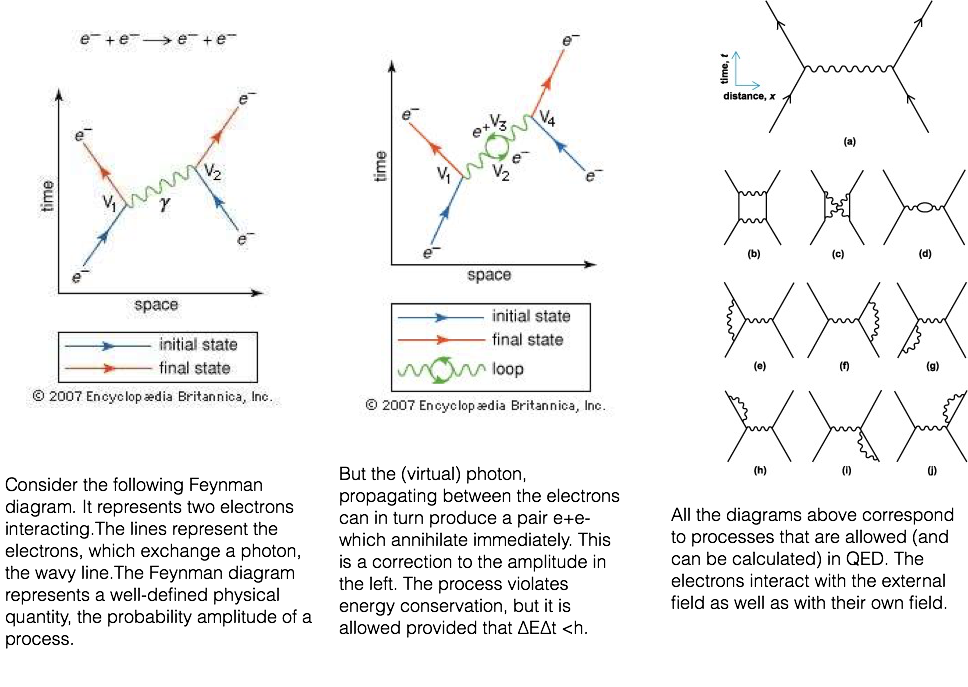
\includegraphics[scale=0.3]{img/FeynmanD3.png}

\end{frame}
%%\begin{frame}
\frametitle{Labeling the spinor states}
Since in reality we deal with positrons with positive energies rather than electrons with negative energy, it is convenient to label the spinors in by physical quantities. Using $\phi$~ for electron spinors and $\chi$~ for positron spinors, we can write the spinor as:
\[
\psi = \mqty(\psi_1 \\ \psi_2 \\ \psi_3 \\ \psi_4) =  \mqty(\phi \\ \chi); \,\,\,
\phi =  \mqty(\phi_1 \\ \phi_2), \,\,\, \chi =  \mqty(\chi_1 \\ \chi_2)
\]
The four plane-wave solutions are now:
\[
\phi e^{-i p\cdot x} \,\,\, \chi e^{i p\cdot x}
\]
\end{frame}

%%\begin{frame}
\frametitle{Solutions of the Dirac equation for massless particles}
Define the right-handed and left-handed components of the Dirac spinor by:
\[
\psi_R = P_R \psi, \,\,\, \psi_L = P_L \psi
\]
with:
\[
P_R = \frac{1 + \gamma_5}{2}, \,\,\, P_L = \frac{1 - \gamma_5}{2}
\]
and
\[
\gamma^5 = i\gamma^0\gamma^1\gamma^2\gamma^3 
\]
which, in the Dirac representation equals:
\[
\gamma^5 = \mqty(\sigma_2 & 0 \\ 0 & -\sigma_2)
\]
Now, set the mass to zero in the Dirac equation, to get: 
\[
i \gamma^\mu \partial_\mu \psi = 0 \, \, \, (m=0)
\]
Then see that $\psi_R$~and $\psi_L$~also satisfy the massless Dirac equation
\end{frame}
\begin{frame}

\[
i \gamma^\mu \partial_\mu \psi_R = i \gamma^\mu P_R \partial_\mu \psi = 
P_L i \gamma^\mu \partial_\mu \psi = 0
\]
and the same result is found exchanging $P_R$~and $P_L$. This means that the right-handed and left-handed spinors satisfy \alert{independently} the Dirac equation. 
\[
i \gamma^\mu \partial_\mu \psi_R = 0 \, \, \, i \gamma^\mu \partial_\mu \psi_L = 0 \, \, \, (m=0)
\]
while if the mass is not zero they cannot be separated. 
\[
(i \gamma^\mu \partial_\mu - m) \psi_R =  i \gamma^\mu \partial_\mu \psi_R -m  \psi_R \ne 0
\]

\end{frame}

\begin{frame}
\frametitle{Weyl representation}
In the Weyl representation, the $\gamma$~matrices are chosen to be:
\[
\gamma^0 = \mqty(0 & I \\ I & 0), \,\,\,  \gamma^1 = \mqty(i \sigma_1 & 0 \\ 0 & i \sigma_1),
\gamma^2 = \mqty(0 & -\sigma_2 \\ \sigma_2 & 0), \,\,\,  
\gamma^3 = \mqty(i \sigma_3 & 0 \\ 0 & i \sigma_3)
\]
\[
\gamma^5 = \mqty(\sigma_2 & 0 \\ 0 & -\sigma_2) =  \mqty(I & 0 \\ 0 & -I)
\]
and 
\[
P_R =  \mqty(I & 0 \\ 0 & 0), \,\,\, P_L =  \mqty(0 & 0 \\ 0 & I)
\]
which means that $P_R$~ filters out the top two components and $P_R$~ filters out the bottom two components. Namely, in the Weyl representation the top half and the bottom half of the spinor transform independently under Lorentz transformations. 
\end{frame}
\begin{frame}
\frametitle{Helicity}
We define the helicity of a particle propagating with momentum $\va{p}$ as the spin projection in the
direction of $\va{p}$:
\[
h =  \frac{\va{\sigma}\cdot \va{p}}{\abs{p}} = (m \rightarrow 0) \gamma_5
\]
and 
\[
P_{R,L} = \frac{1 \pm \gamma_5}{2}
\]
\begin{itemize}
\item represents the helicity $\pm$~�projection operator for $e^-$.
\item represents the helicity $\mp$~�projection operator for $e^+$.
\end{itemize}

Since $\gamma_5$ and any (proper) Lorentz transformation  commute, once a state is an eigenstate of $\gamma_5$, one cannot change the eigenvalue of $\gamma_5$ by boosting it or rotating it.

\end{frame}

\begin{frame}
\frametitle{Masless particles have well defined helicity}
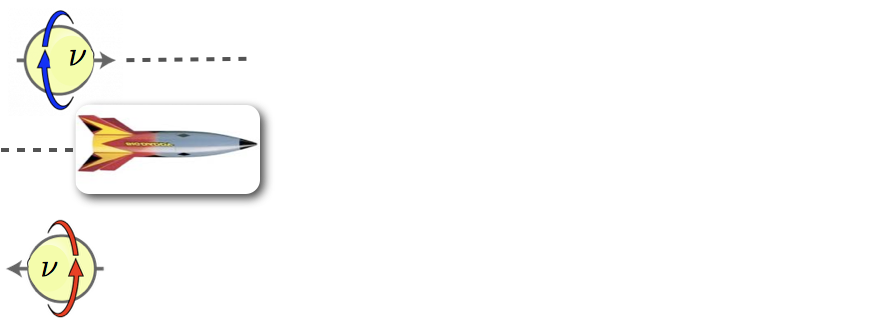
\includegraphics[scale=0.3]{neutrinoBoost2.png}

Namely, in the massless limit, one cannot change the value of helicity by boosting or rotating. This can be understood intuitively. The only way to reverse the spin component along the motion is for the observer to move faster than the particle and overtake it. Then, the direction of momentum viewed by the observer will flip while the spin will stay the same, and thus the helicity will change its sign. In the massless limit, the particle will be moving at the speed of light, and thus it is impossible to overtake it.

\end{frame}

\begin{frame}
\frametitle{Almost massless particles?}
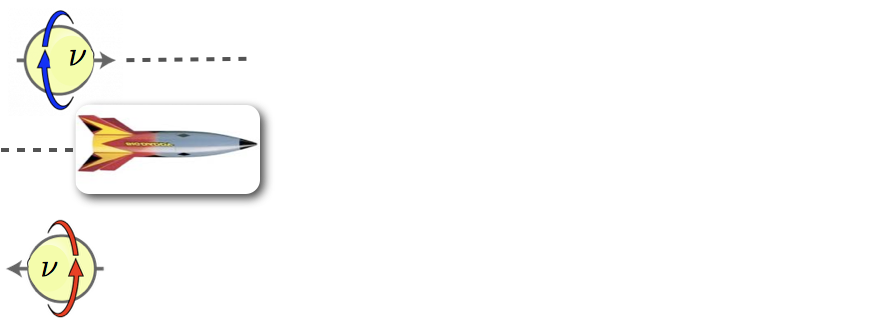
\includegraphics[scale=0.3]{neutrinoBoost2.png}

Experiments have established that the neutrino has a tiny mass. Thus, it moves ``almost'', but not quite at the speed of light, and one can reverse the argument before and jump into a boost that  ``overtakes'' the neutrino, thus see its helicity flip. Yet, the amount of ``wrong'' helicity that each one of the Weyl spinors has is very small, of the order $\frac{m}{E}$, where $m$~is the neutrino mass and $E$~its energy. 

\end{frame}


\begin{frame}
\frametitle{Fermi Theory}

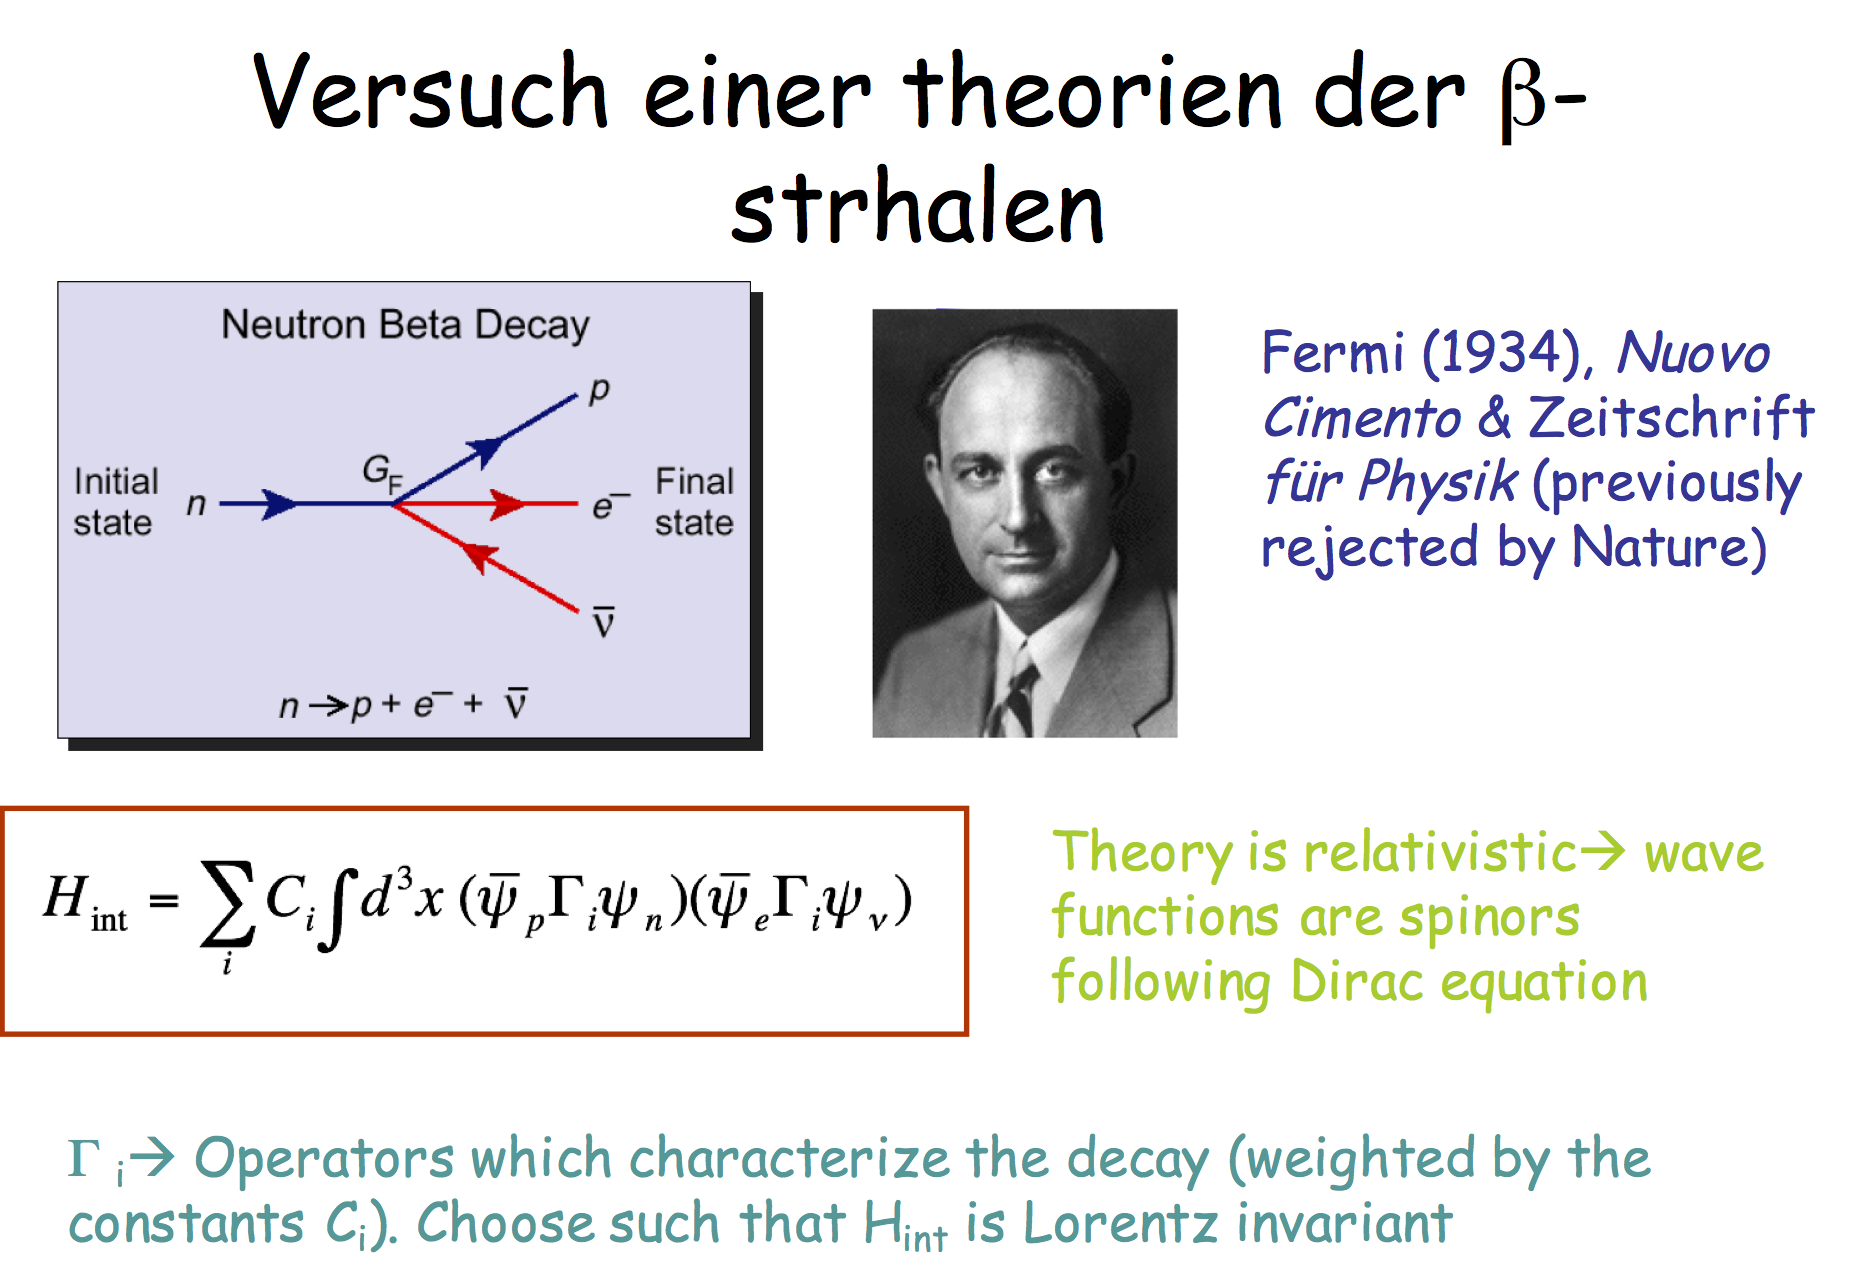
\includegraphics[scale=0.3]{img/FermiTheory.png}

\end{frame}

\begin{frame}
\frametitle{The modern picture of Beta decay}

\includegraphics[scale=0.35]{img/BetaDecay.png}

\end{frame}
\begin{frame}
\frametitle{I do not believe in neutrinos}
\begin{columns}
\column{0.35\textwidth}
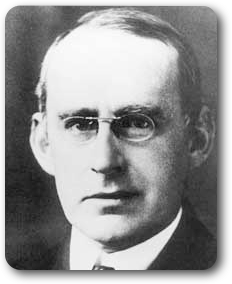
\includegraphics[scale=0.3]{eddington.png}
 
 \column{0.6\textwidth}
%\begin{block}{}
Sir Arthur Eddington: ``Just now nuclear physicists are writing a great deal about hypothetical particles called neutrinos supposed to account for certain peculiar facts observed in $\beta$-ray disintegration. We can perhaps best describe the neutrinos as little bits of spin-energy that have got detached. I am not much impressed by the neutrino theory. \alert{In an ordinary way I might say that I do not believe in neutrinos}... But I have to reflect that a physicist may be an artist, and you never know where you are with artists. My old-fashioned kind of disbelief in neutrinos is scarcely enough. \alert{Dare I say that experimental physicists will not have sufficient ingenuity to make neutrinos?"}

%\end{block}
\end{columns}
\end{frame}

\begin{frame}
\frametitle{The discovery of neutrinos}

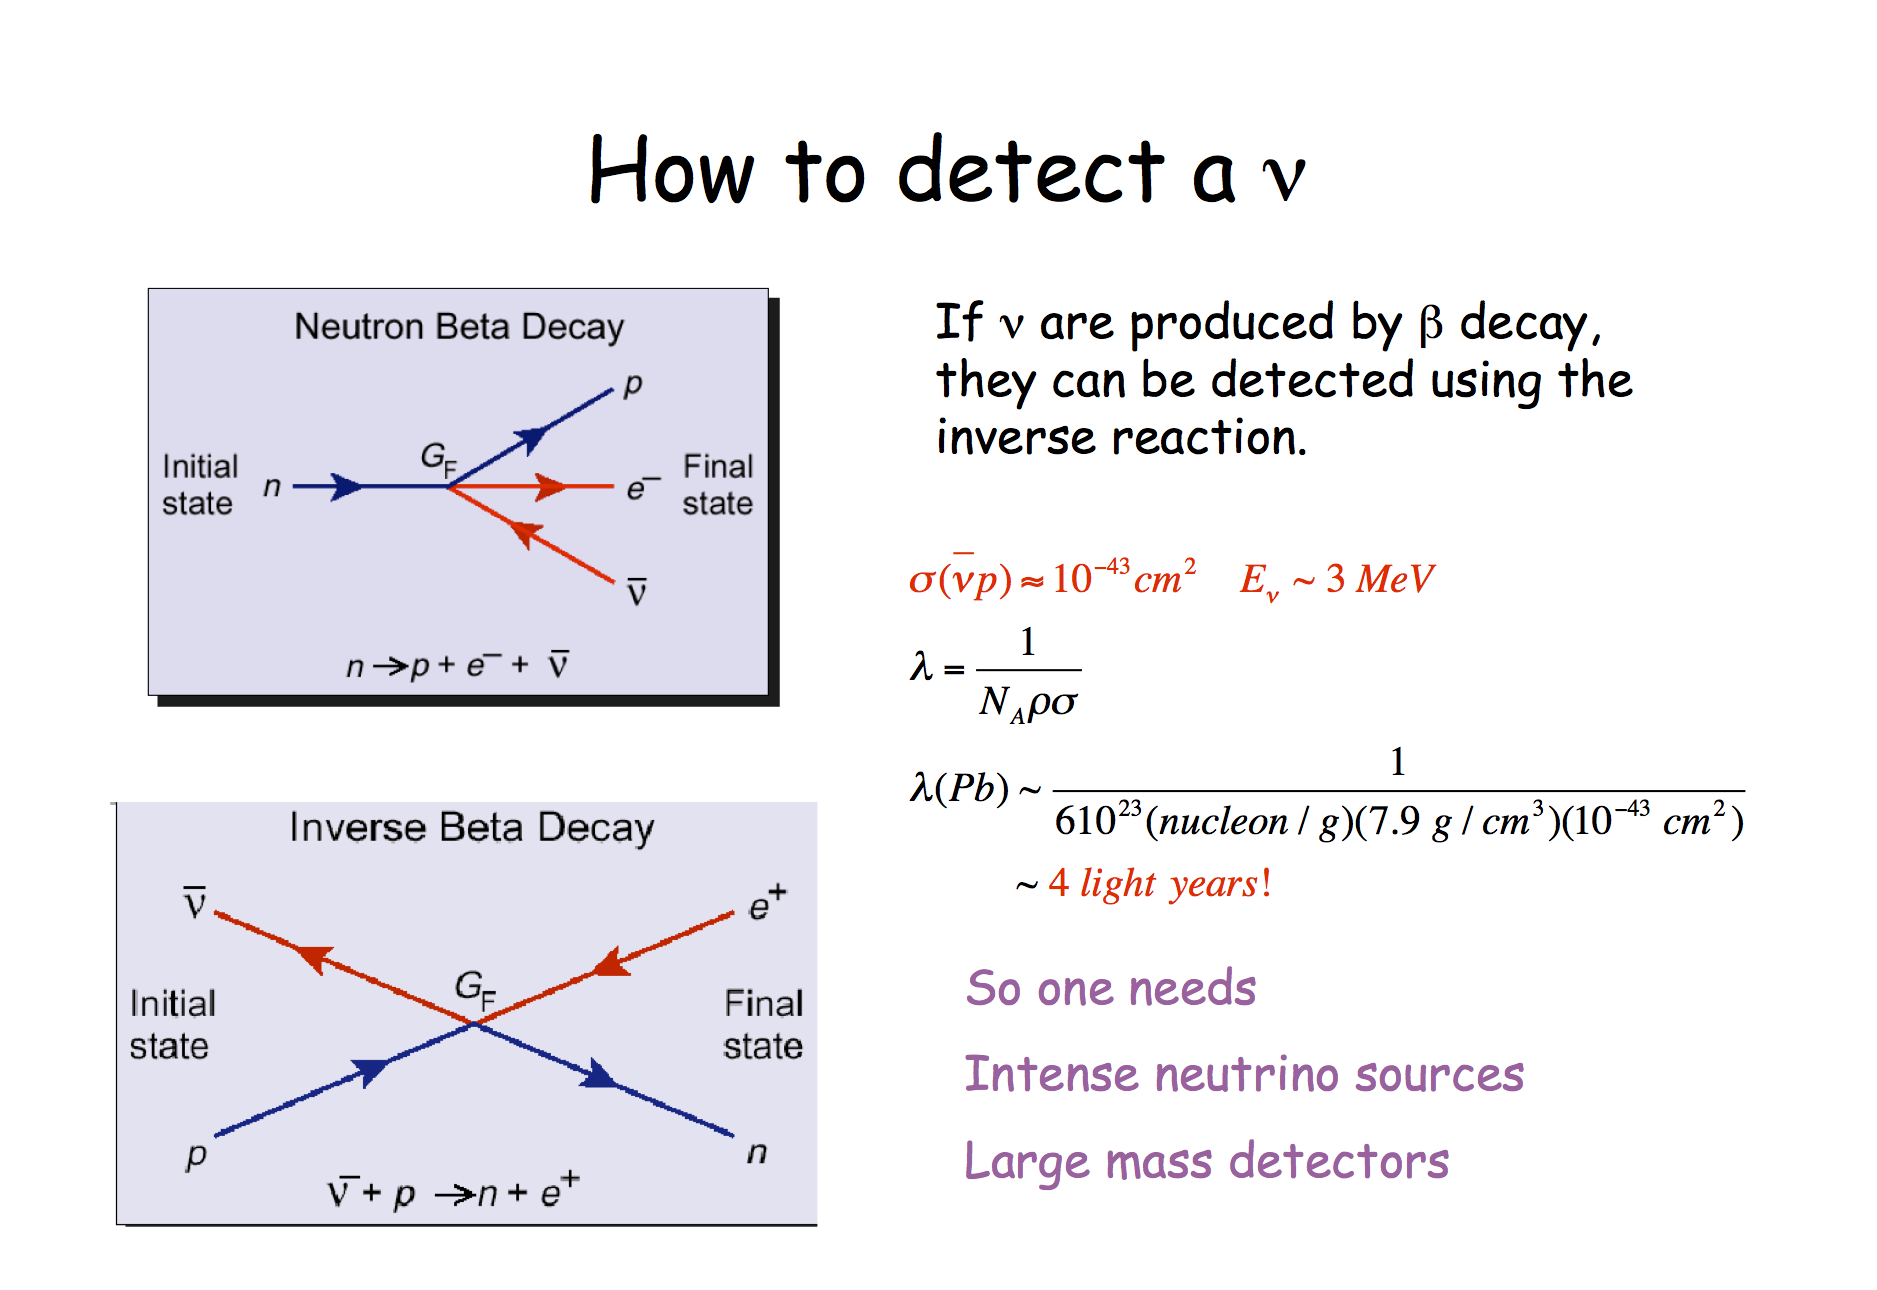
\includegraphics[scale=0.3]{DetectNeutrinos.png}

\end{frame}

\begin{frame}

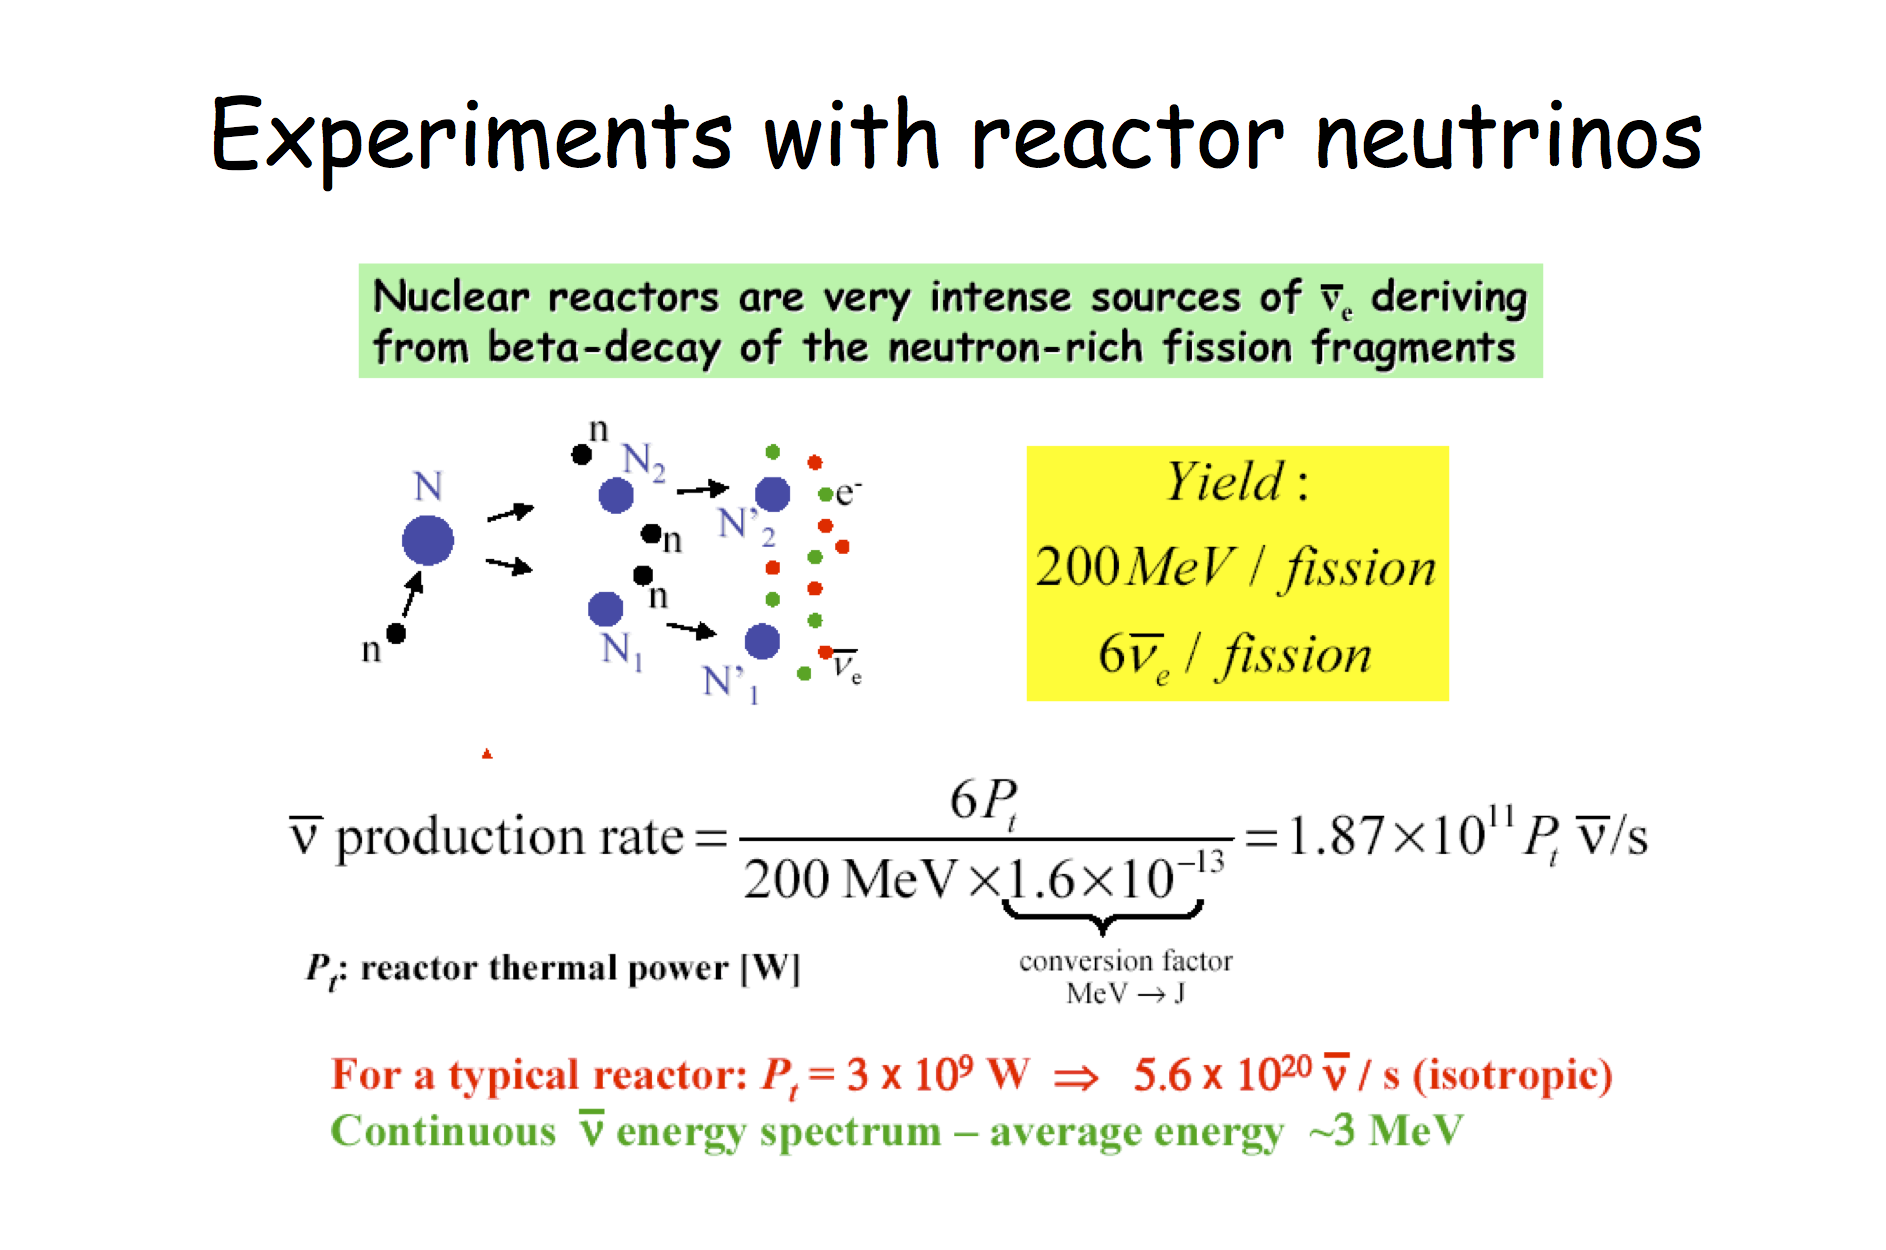
\includegraphics[scale=0.35]{ReactorNeutrinos.png}

\end{frame}

\begin{frame}

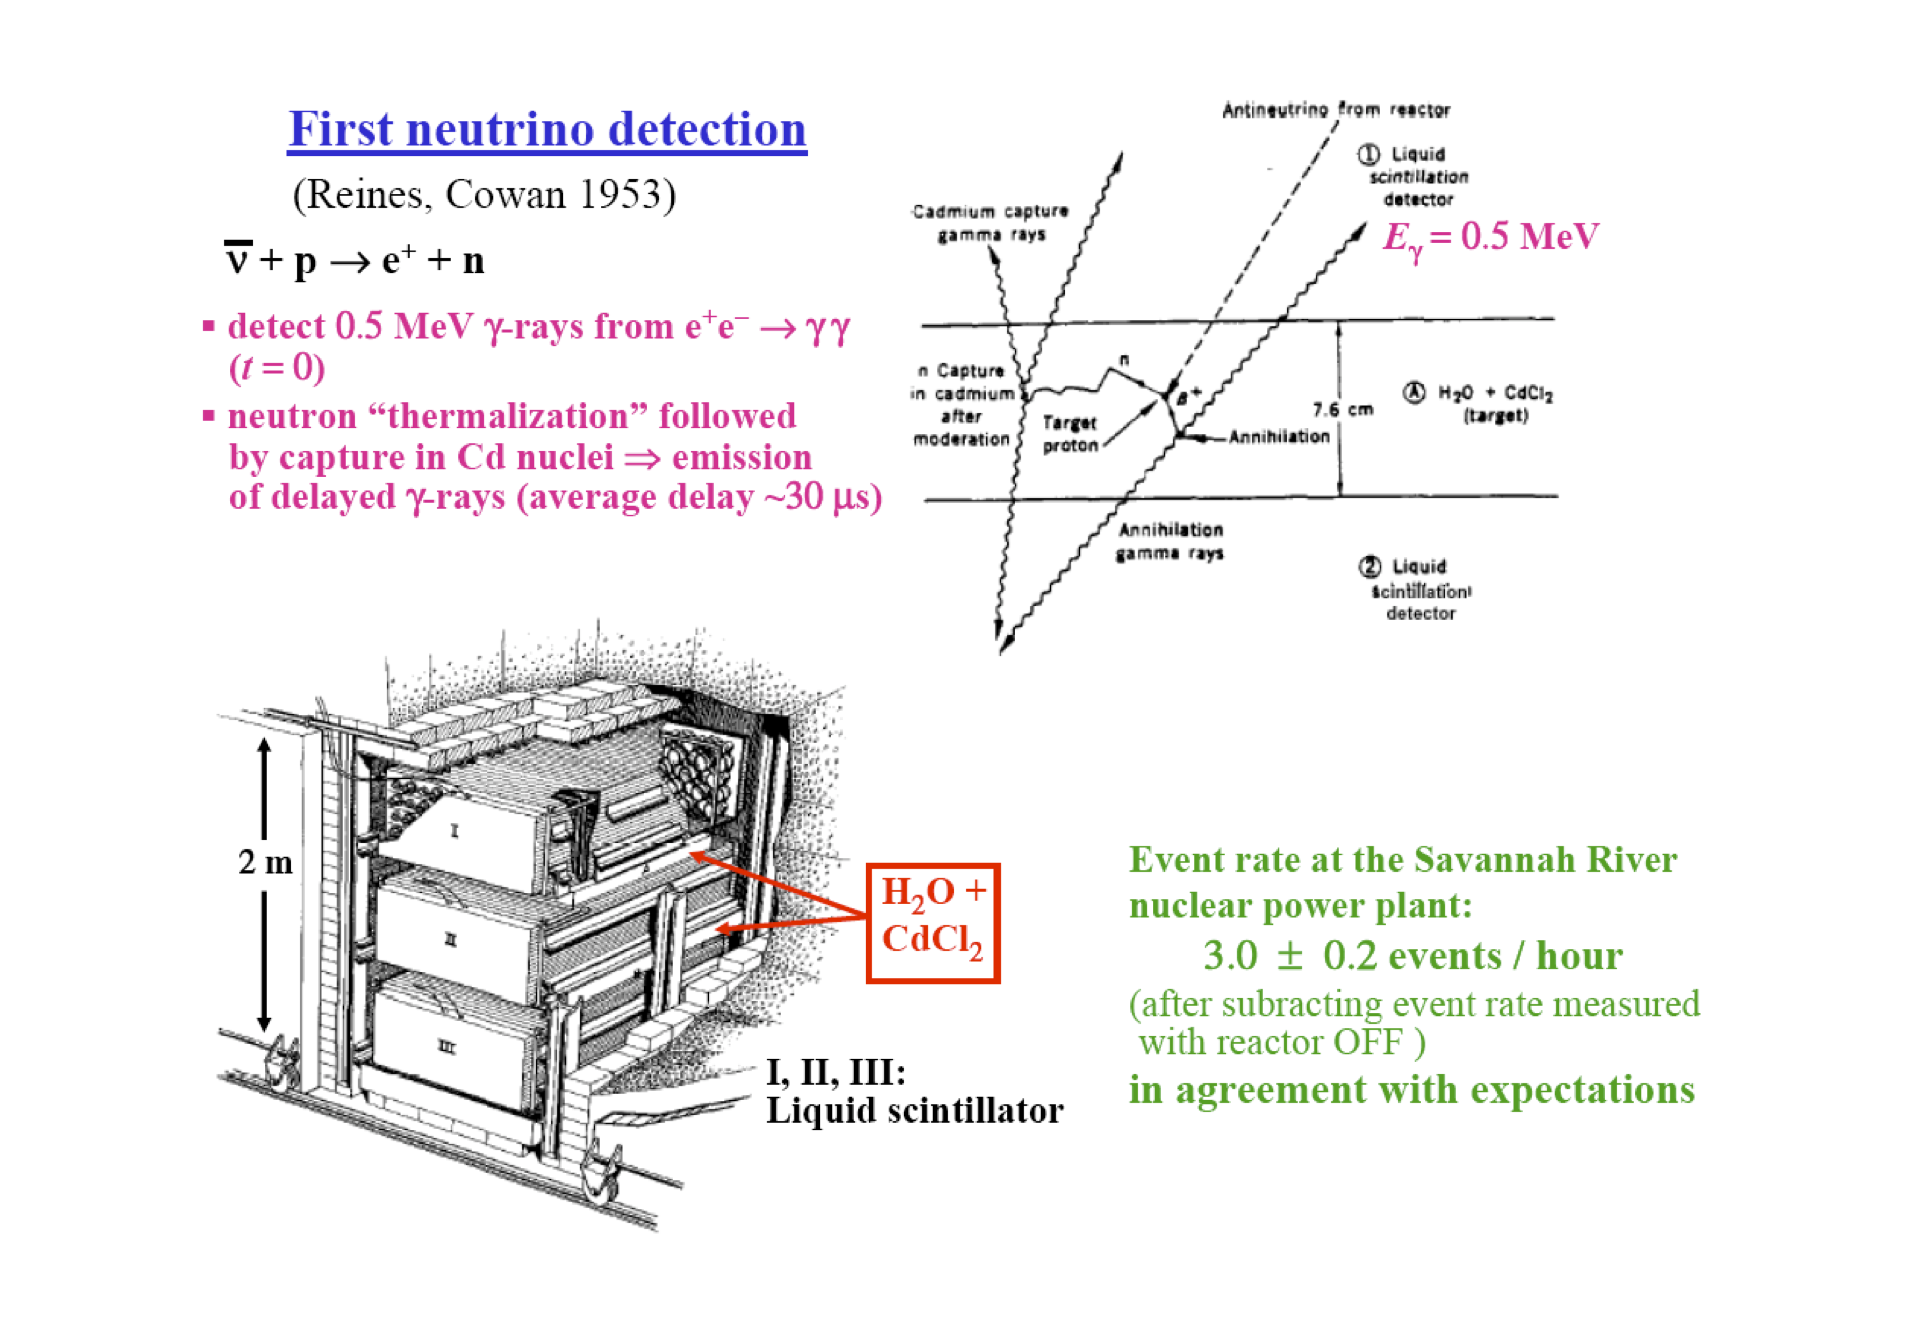
\includegraphics[scale=0.35]{FirsNeutrino.png}

\end{frame}

%\begin{frame}
%
%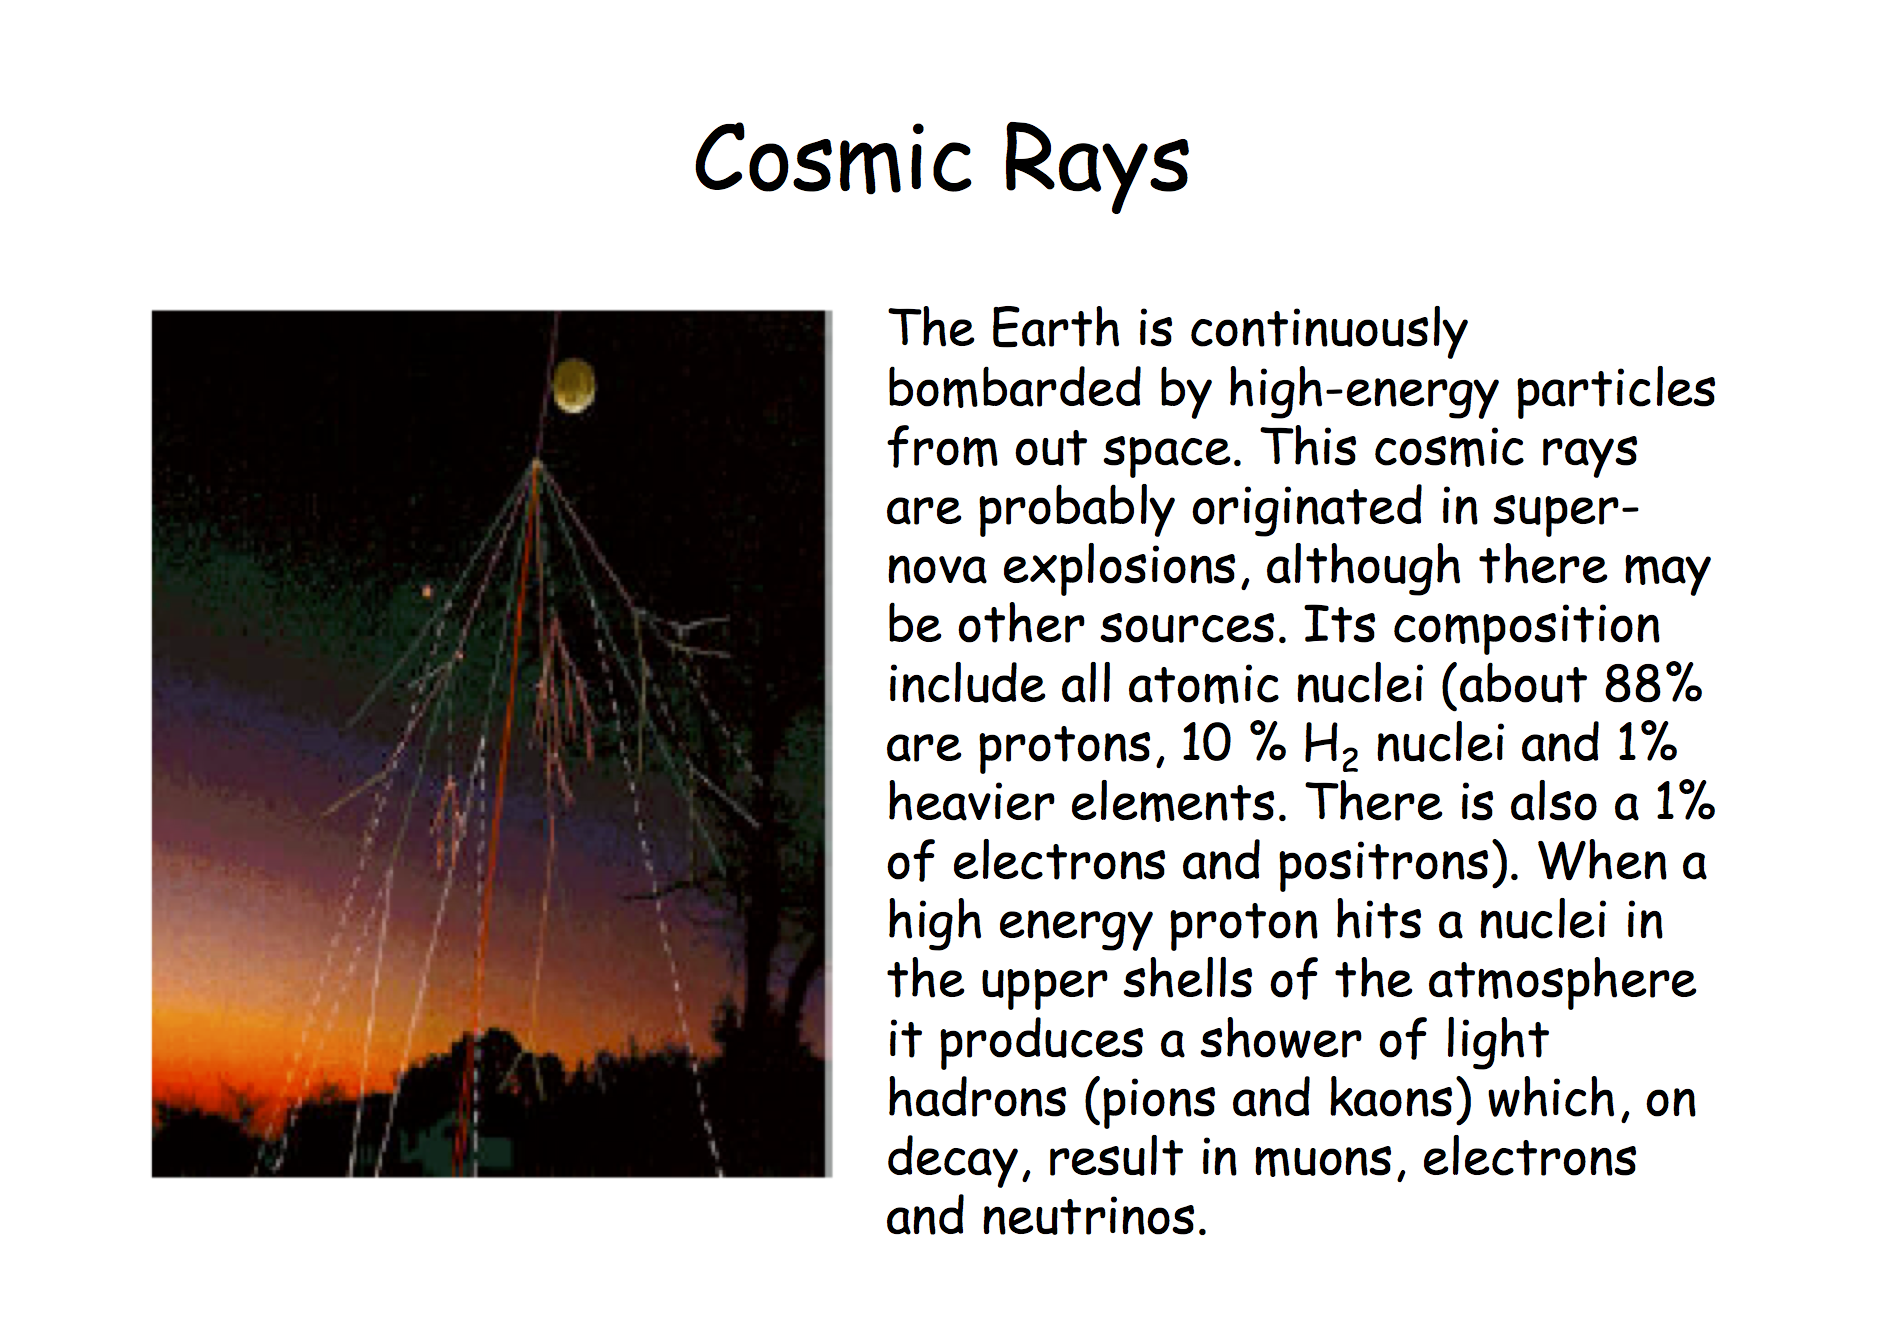
\includegraphics[scale=0.35]{CosmicRays.png}
%
%\end{frame}
%\begin{frame}
%
%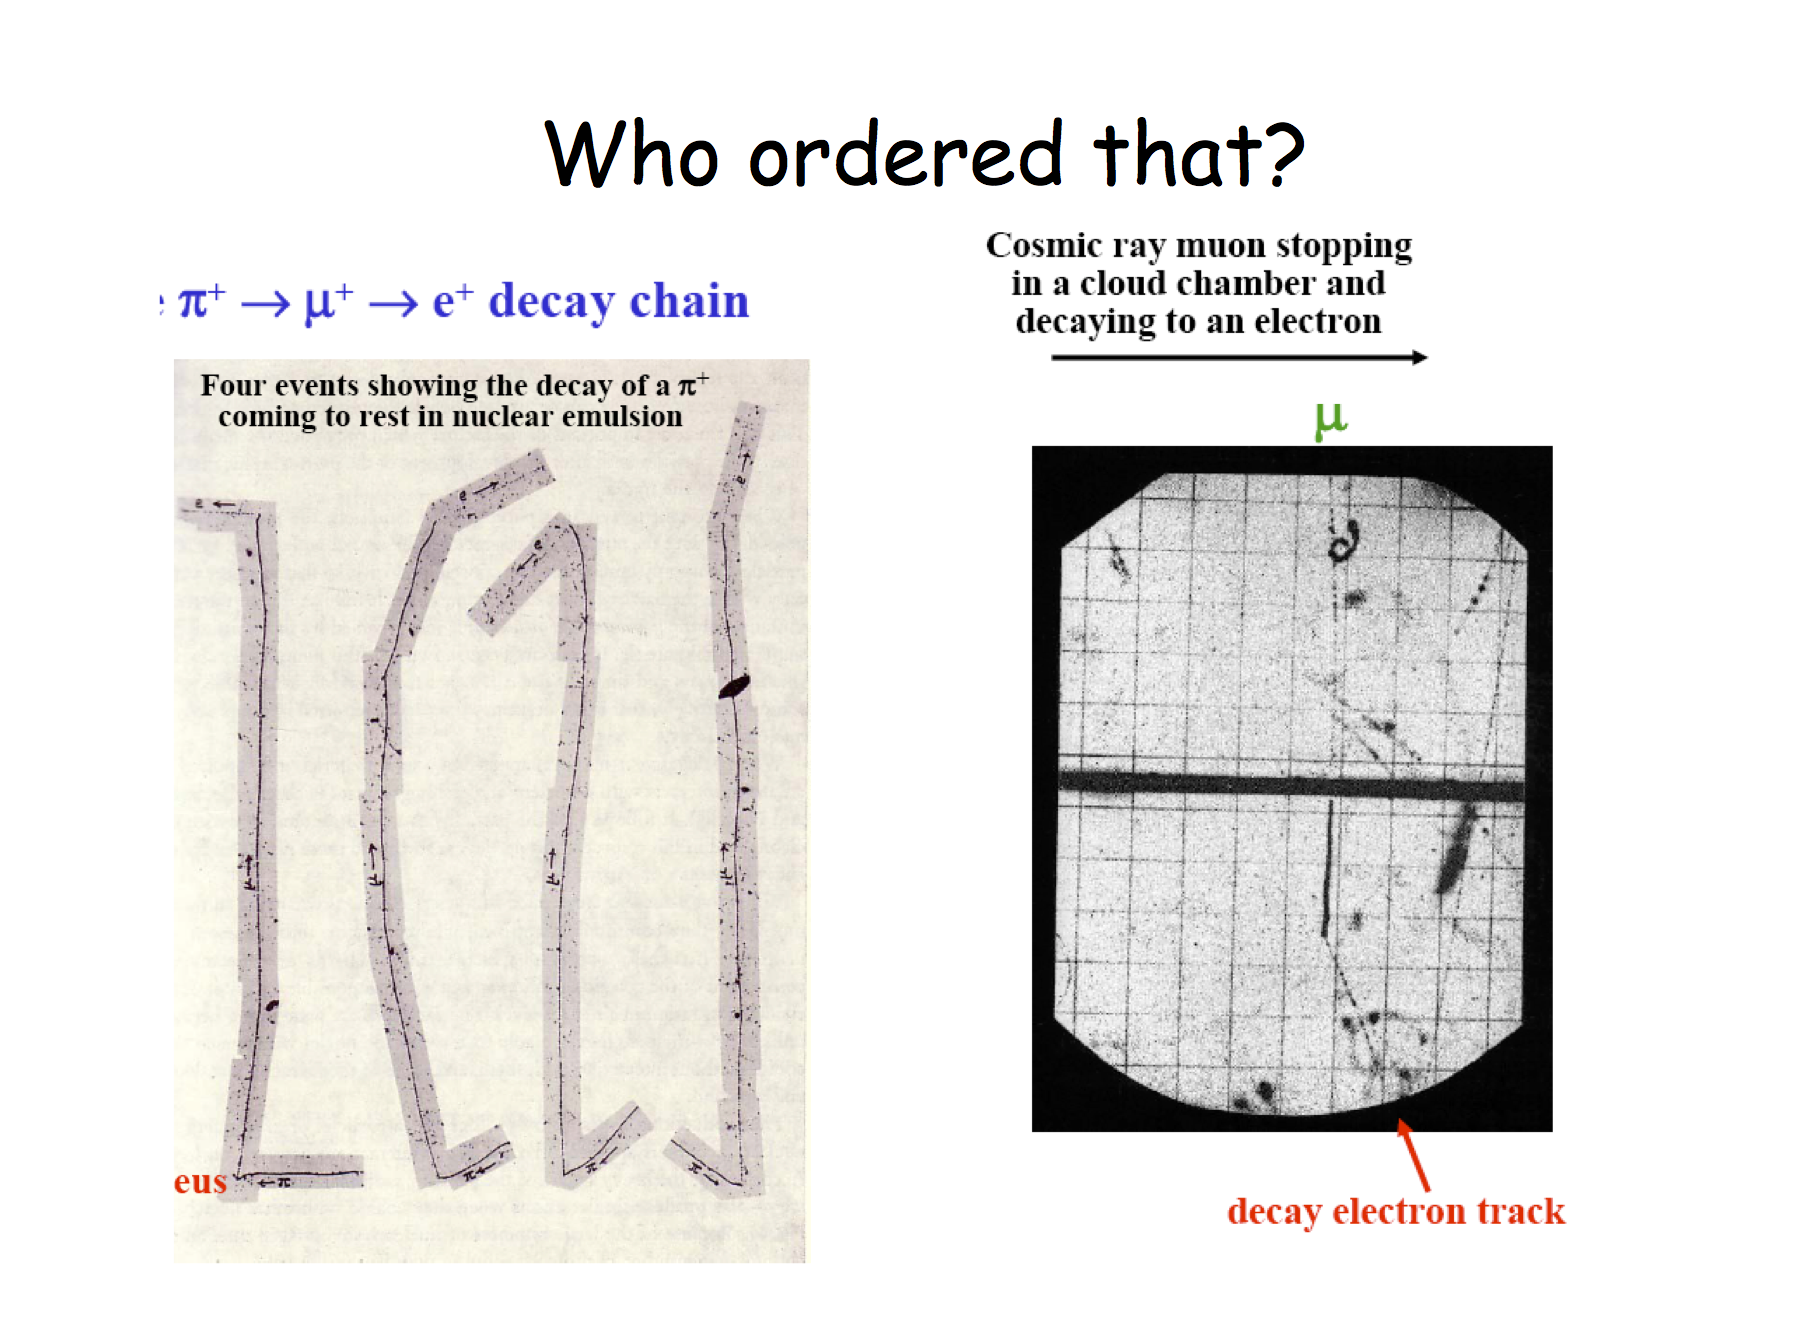
\includegraphics[scale=0.35]{WhoOrderedThat.png}
%
%\end{frame}
%\begin{frame}
%
%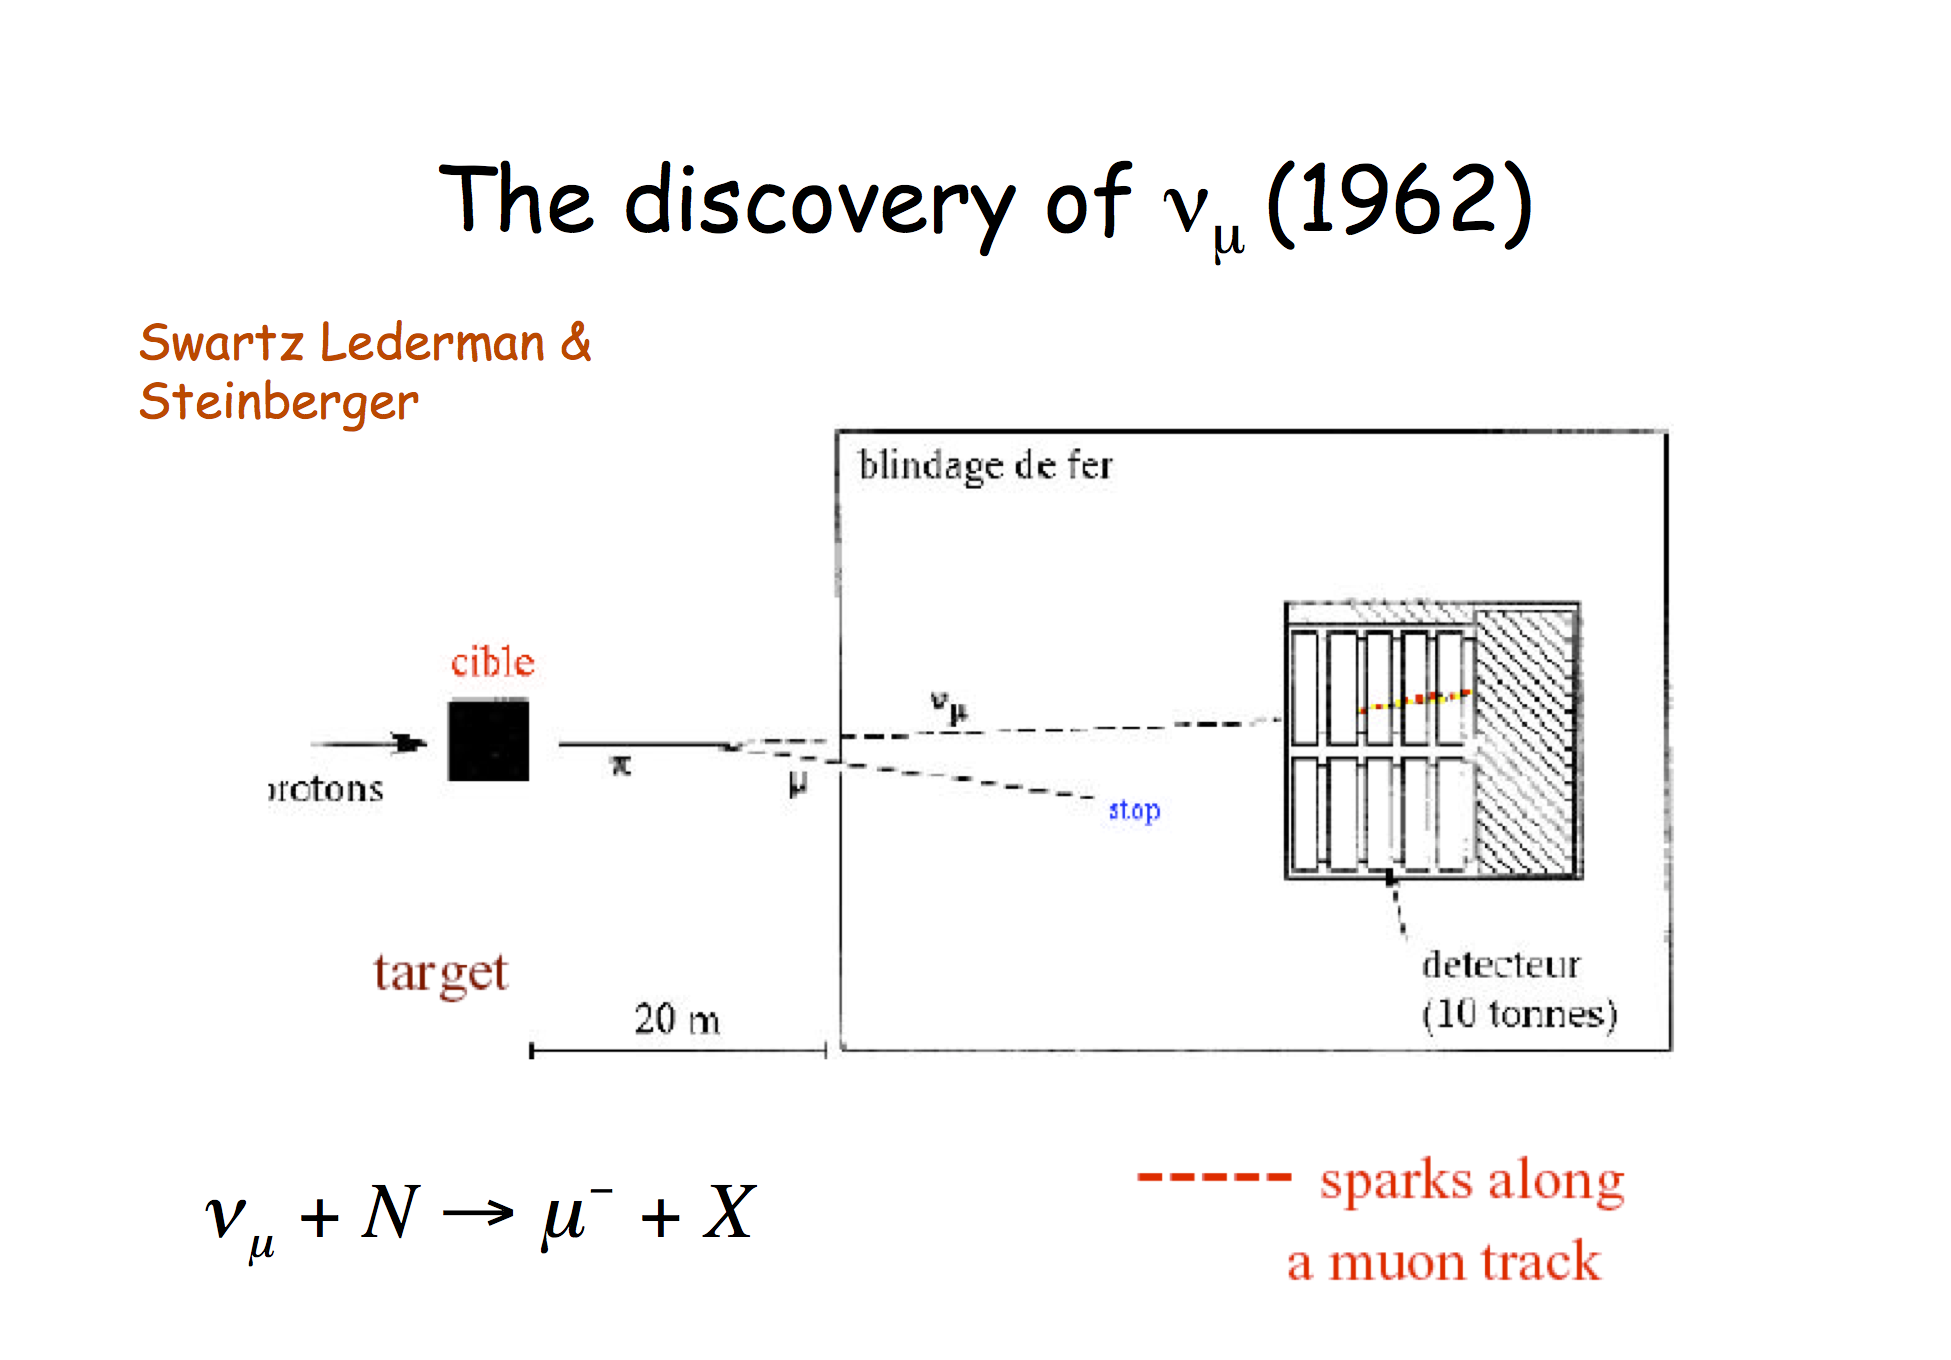
\includegraphics[scale=0.35]{DiscoveryNumu.png}
%
%\end{frame}
%\begin{frame}
%
%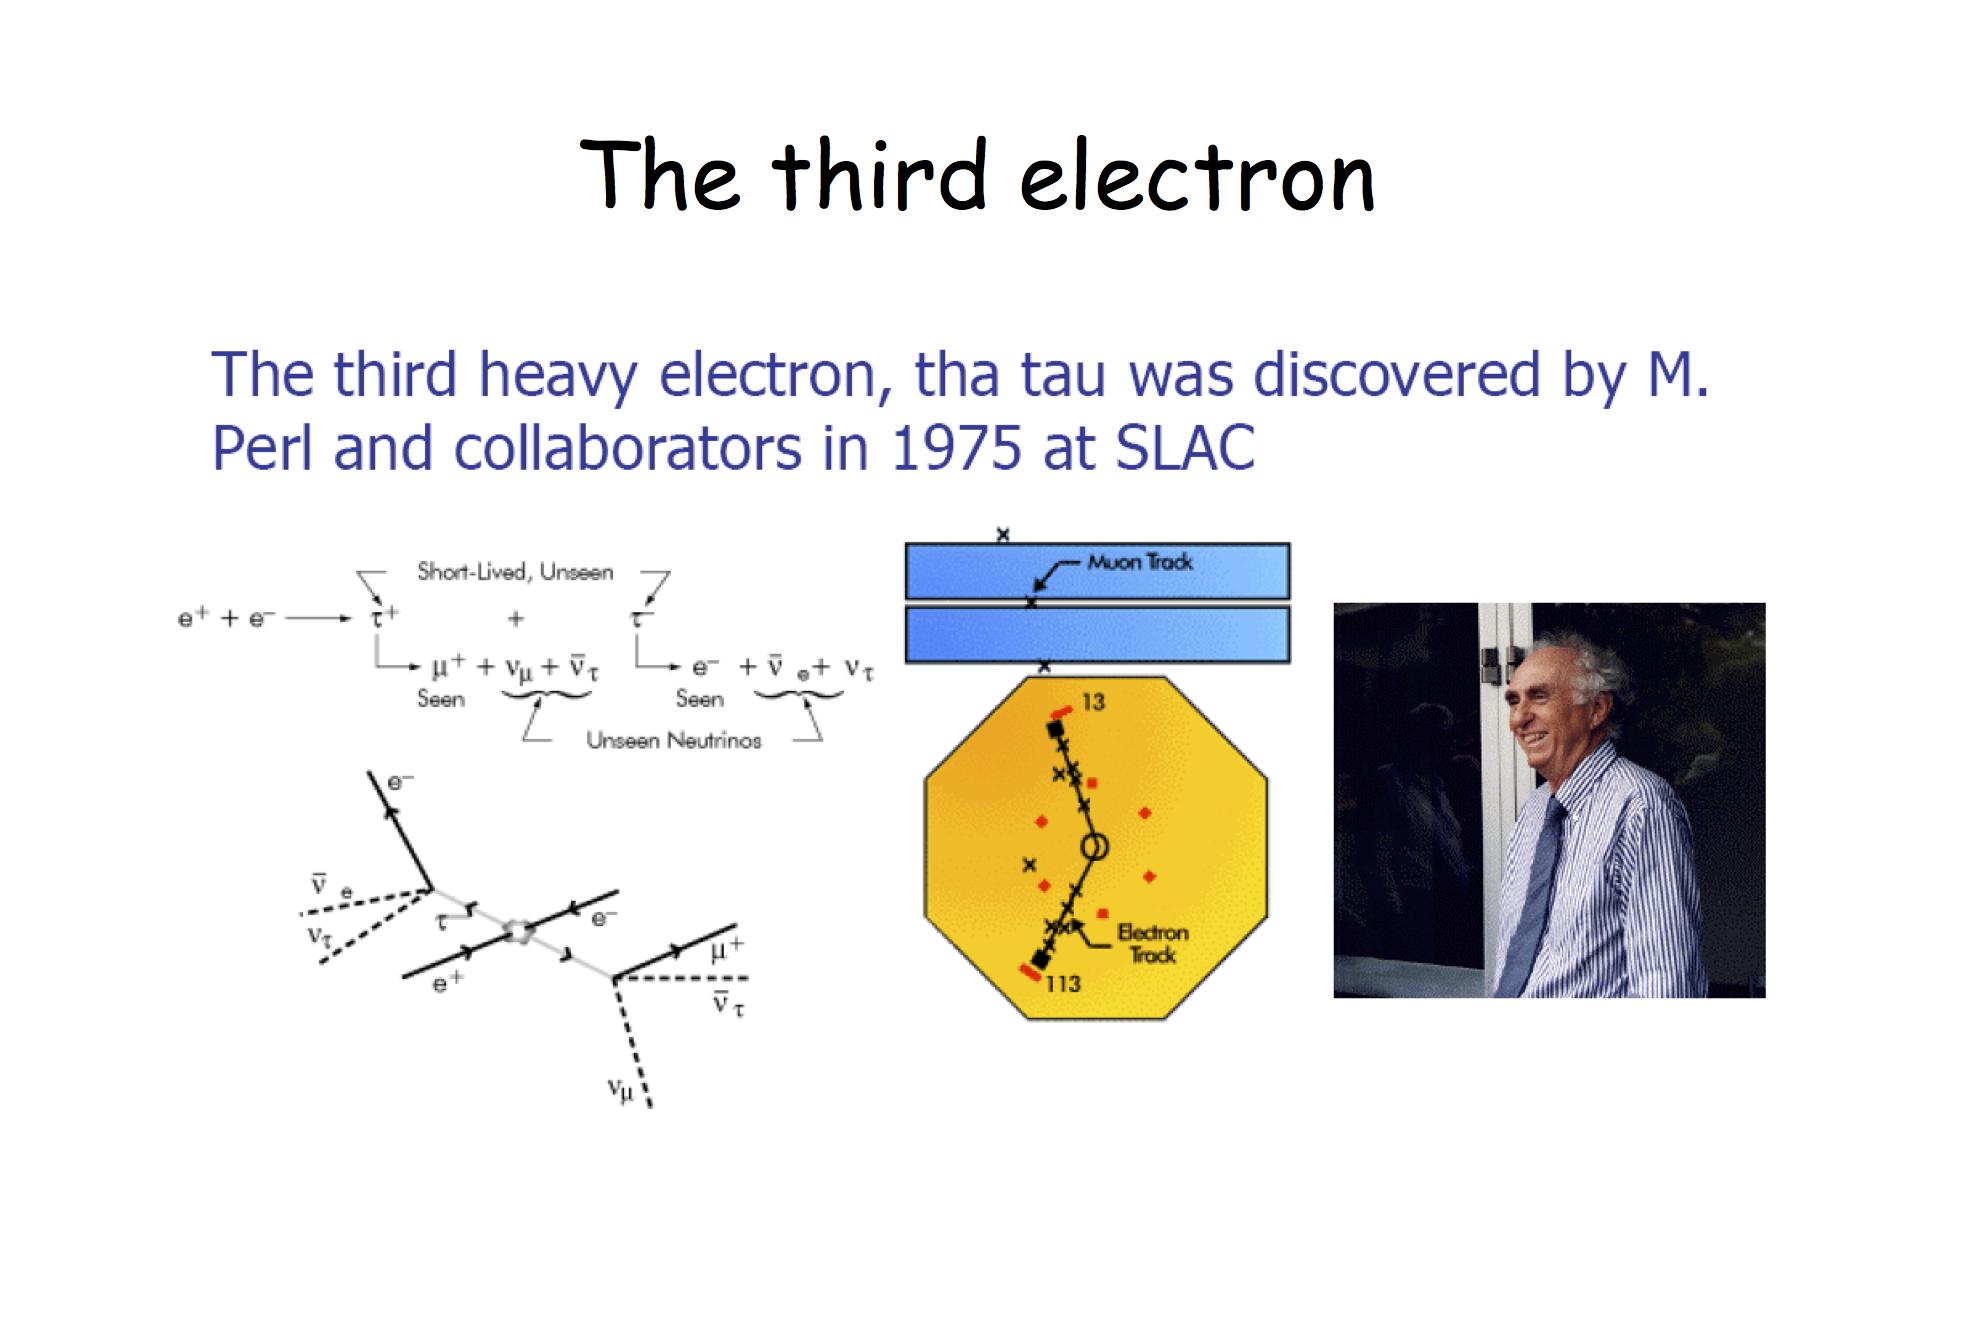
\includegraphics[scale=0.35]{tau.png}
%
%\end{frame}
%\begin{frame}
%
%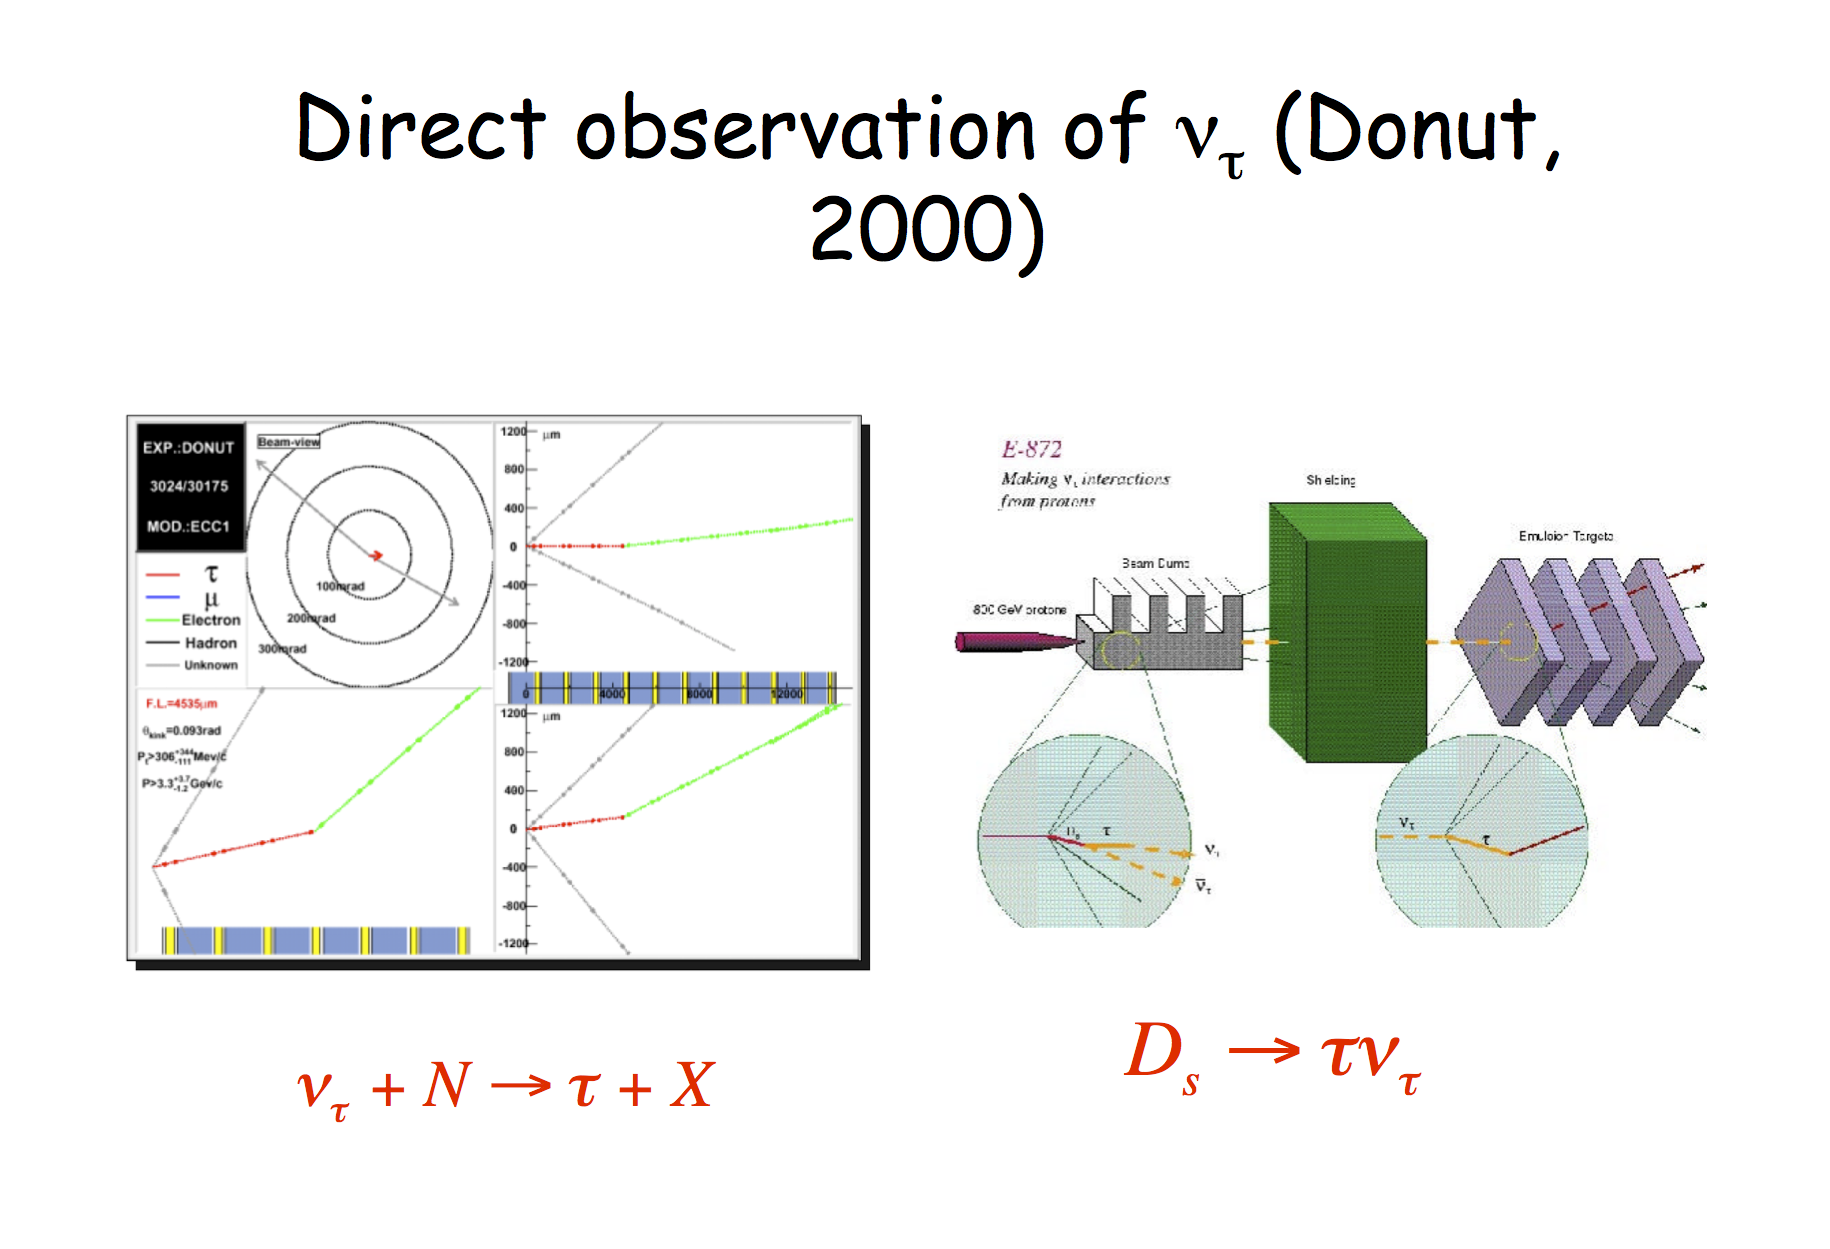
\includegraphics[scale=0.35]{DirectNuTau.png}
%
%\end{frame}
\begin{frame}
\frametitle{Neutrinos everywhere}
\begin{columns}
\column{0.35\textwidth}
\includegraphics[scale=0.25]{Generations2.png}

Two heavy electrons (the $\mu$~and the $\tau$) have been discovered, each one accompanied with its own neutrino. For reasons yet unknown to us, Nature has chosen to produce three copies of the elementary fermions, identical except for their mass. 
 
 \column{0.6\textwidth}
%\begin{block}{}
\includegraphics[scale=0.25]{NeutrinoSources.png}

Neutrinos are everywhere and we have produced and detected them by the millions. Eddington would not have made a living as a prophet (who does?)


%\end{block}
\end{columns}




\end{frame}


\begin{frame}
\frametitle{Neutrinos through the looking glass}

\includegraphics[scale=0.4]{Alice.png}

\end{frame}


\begin{frame}
\frametitle{Parity}
\begin{columns}
\column{0.5\textwidth}
\includegraphics[scale=0.45]{ParityCartoon.png}


The parity transformation changes a right-handed coordinate system into a left-handed one or vice versa. Two applications of the parity transformation restores the coordinate system to its original state.

It is a reasonable presupposition that nature should not care whether its coordinate system is right-handed or left-handed, \alert{but surprisingly, that turns out not to be so.}

\column{0.5\textwidth}
%\begin{block}{}
\includegraphics[scale=0.35]{wu.png}

In 1956, T. D. Lee and C. N. Yang predicted the non conservation of parity in the weak interaction. Their prediction was quickly tested when C. S. Wu and collaborators studied the beta decay of Cobalt-60 in 1957.

%\end{block}
\end{columns}

\end{frame}

%\begin{frame}
%\includegraphics[scale=0.35]{Cobalt.png}
%%wu.png
%\end{frame}
%GoldhaberExperiment.png
\begin{frame}
\includegraphics[scale=0.35]{Goldhaber.png}

\end{frame}

\begin{frame}
\frametitle{What do we talk about when we talk about helicity?}
\begin{columns}
\column{0.5\textwidth}
\includegraphics[scale=0.35]{NeutrinoHelicity.png}

Helicity is the spin projection in the direction of motion.
\[
h = \frac{\va{\sigma}\cdot \va{p}}{p}
\]
The Goldhaber experiment measured that neutrinos are left handed (spin opposed to motion, $h=-1$). The CPT theorem ensures that anti-neutrinos must be right-handed (spin along motion, $h=+1$).
\column{0.5\textwidth}

\includegraphics[scale=0.30]{neutrinoBoost2.png}

For massive particles, helicity depends on the reference frame and thus is not Lorentz invariant. One can always jump into a reference system faster than that of the particle and see its helicity flip.

But massless particles travel at the speed of light and cannot be overtaken. The helicity becomes a constant of motion. 
\end{columns}

\end{frame}

%
%\begin{frame}
%\includegraphics[scale=0.35]{AntineutrinosRH.png}
%
%\end{frame}

%\begin{frame}
%\frametitle{What do we talk about when we talk about (Standard Model) neutrinos?}
%\includegraphics[scale=0.90]{NeutrinoOverview.png}
%\end{frame}

\begin{frame}
\frametitle{Neutrinos through the looking glass}
\includegraphics[scale=0.33]{NeutrinosLookingG.png}
\end{frame}

\begin{frame}
\frametitle{But what if neutrinos are massive}
\includegraphics[scale=0.33]{WhatIfNeutrinoMassive.png}
WhatIfNeutrinoMassive.png

\end{frame}





\begin{frame}
\frametitle{A symmetric electron-positron theory (1937)}
\begin{columns}
\column{0.35\textwidth}
\includegraphics[scale=0.32]{img/MajoranaPaper.png}
\column{0.35\textwidth}
We show that it is possible to achieve complete formal symmetrization in the electron and positron quantum theory by means of a new quantization process. The meaning of Dirac equations is somewhat modified and {\bf it is no more necessary to speak of negative-energy states; nor to assume, for any other type of particles, especially neutral ones, the existence of antiparticles, corresponding to the ``holes'' of negative energy.}
\end{columns}
\end{frame}

%\begin{frame}
%\frametitle{An unpleasant symmetry}
%\begin{itemize}
%\item ``The interpretation of the so called ``negative energy states'' proposed by Dirac leads, as it is well known, to a substantially symmetric description of electron and positrons... but it looks to us important, in view of possible extensions, that the notion itself of negative energy state be abandoned." 
%\item ``Indeed, we shall see that to be perfectly possible to build, in the most natural way, a theory of the neutral elementary particles without negative states."
%\item ``The new approach allows not only to give a symmetric form to the electron-positron theory, but also to build a substantially novel theory for the particles deprived of electric charge."
%\item ``it is probably not yet possible to ask to the experience to decide between this new theory and the simple extension of the Dirac equations to the neutral particles."
%\end{itemize}
% 
% \alert{VOW!}
% 
%\begin{itemize}
%\item At the time the neutrino had not yet been discovered. 
%\item Even if in those times the only known ``charge'' was the electric charge, Majorana implicitly assumed particles deprived of \alert{all the possible charges}. 
%%\item Eighty years later we have not yet been able to decide between Dirac and Majorana theories.
%%\item But we hope we will be able to tell in maybe another ten or twenty years.
%\end{itemize}
%\end{frame}

%\begin{frame}
%\frametitle{Majorana's approach}
%Majorana questioned whether it was necessary for spin-1/2 particles to have equations that involved complex numbers. What was required were gamma matrices that still satisfy the Clifford algebra but were purely imaginary. Majorana found such constructions in terms of the Pauli matrices:
%\[
%\gamma^0 = \mqty(0 & \sigma_2 \\ \sigma_2 & 0), \,\,\,
%\gamma^1 = \mqty(i \sigma_1 & 0 \\ 0 & i \sigma_1), \,\,\,
%\gamma^2 = \mqty(0 & -\sigma_2 \\ \sigma_2 & 0), \,\,\,
%\gamma^4 = \mqty(i \sigma_3 & 0 \\ 0 & i \sigma_3)
%\]
%Recall that $\sigma_1, \sigma_3$~are real, while $\sigma_2$~is complex. Thus, all the Majorana gamma matrices are complex. But then, the Majorana spinor $\psi_M$~must be real \alert{and is therefore invariant to charge conjugation}. The derived field theory can be constructed from one type of operator. Therefore, the particles created \alert{are fermions that are their own antiparticles}.
%\end{frame}

\begin{frame}
\frametitle{Dirac revisited}
Recall the Dirac equation:
\[
(i \gamma^\mu \partial_\mu -m ) \psi  = 0
\]
which we can rewrite (using $i \partial_0 \rightarrow E, i \partial_i \rightarrow - \va{p}$) as:
\[
(E - \va{p}\cdot\va{\sigma} - m ) \psi  = 0
\]
Also recall that $\psi$~is a 4-dimensional spinor:
\[
\psi = \mqty(\psi_1 \\ \psi_2 \\ \psi_2 \\ \psi_4) = \mqty(\phi \\ \chi)
\]
where $\phi =  \mqty(\phi_1 \\ \phi_2)$ represents a particle (with two spin states) and
$\chi =  \mqty(\chi_1 \\ \chi_2)$ represents an antiparticle (also with two spin states).
\end{frame}

\begin{frame}
\frametitle{Dirac equation using Weyl representation of the $\gamma$~matrices}
\[
\gamma^0  = \mqty(0 & I \\ I & 0),\,\,\, \gamma^i  = \mqty(0 & -\sigma^i \\ \sigma^i  & 0)
\]
Then the Dirac equation becomes:
\[
\left[ E  \mqty(0 & I \\ I & 0) - \mqty(0 & -\va{p}\cdot\va{\sigma} \\ \va{p}\cdot\va{\sigma}  & 0) -m \right]
 \mqty(\phi \\ \chi) = 0
\]
which solves into two equations:
 \begin{empheq}[box=\fbox]{align}
(E +  \va{p}\cdot\va{\sigma}) \chi - m \phi & = 0 \nonumber \\
(E -  \va{p}\cdot\va{\sigma}) \phi - m \chi & = 0 \nonumber
\end{empheq}

In the limit of $m \rightarrow 0$~ these two equations decouple and we obtain
two states with definite helicity:
 \begin{empheq}[box=\fbox]{align}
(E +  \va{p}\cdot\va{\sigma}) \chi  & = 0 \nonumber \\
(E -  \va{p}\cdot\va{\sigma}) \phi  & = 0 \nonumber
\end{empheq}
Notice that we have now only two degrees of freedom, since the particle has negative helicity and the antiparticle positive helicity. 
\end{frame}


\begin{frame}
\frametitle{Majorana insight}
Majorana proposed an alternative to the two-coupled, two-component Dirac equation, namely two independent, relativistic, two-component equations:

 \begin{empheq}[box=\fbox]{align}
(E +  \va{p}\cdot\va{\sigma}) \chi - m \epsilon \chi^* & = 0 \nonumber \\
(E -  \va{p}\cdot\va{\sigma}) \phi - m \epsilon \phi^* & = 0 \nonumber
\end{empheq}
where
\[
\epsilon = i \sigma_2 = \mqty(0 & I \\ -I & 0)
\]
If we compare the Dirac and Majorana equations:
\begin{eqnarray*}
(E +  \va{p}\cdot\va{\sigma}) \chi - m \phi & = &  0 \\
(E +  \va{p}\cdot\va{\sigma}) \chi - m \epsilon \chi^* & = & 0
\end{eqnarray*}
It's obvious that both equations are identical for $m=0$. In the Standard Model neutrinos are assumed to be massless and thus both theories are identical. Instead, if neutrinos are massive they are not. The remarkable thing about Majorana equation is that it is constructed only with the $\phi$ (or the $\chi$ for the second equation), thus eliminating two degrees of freedom. 
\end{frame}

\begin{frame}
\frametitle{Is the neutrino its own antiparticle?}
\alert{A particle is its own antiparticle if we can reverse all its charges without effect}. Obviously electrons cannot be their own antiparticles, but Dirac neutrinos are also not their own antiparticles, as explicit in the construction of the bi-spinor that separates particles ($\phi$) and antiparticles ($\chi$).

Given a spinor $\phi$~representing a particle, the charge-conjugate spinor representing an antiparticle is:

 \begin{empheq}[box=\fbox]{align}
 \phi^C & = C \gamma^0 \phi^*\nonumber
\end{empheq}
%\[
%\phi^C = C \gamma^0 \phi^* 
%\]
where $\phi^*$~is the complex conjugate of $\phi$ and the charge conjugation matrix $C$~can be written in the Weyl representation as:
\[
C = \mqty(-i\sigma_2 & 0 \\ 0 & i\sigma_2), \,\,\, C \gamma^0 = \mqty(0 & -i\sigma_2 \\ i \sigma_2 & 0)
\] 
\end{frame}

\begin{frame}
For a Majorana spinor $\phi  \mqty(\phi \\ i \sigma_2 \phi^*)$:
\begin{empheq}[box=\fbox]{align}
\phi^C & = C \gamma^0 \phi^* =  \mqty(0 & -i\sigma_2 \\ i \sigma_2 & 0) \mqty(\phi^* \\ -i \sigma_2 \phi) \\
& =\mqty(-i^2 \sigma^2 \phi \\ i \sigma_2 \phi^*) = \mqty(\phi \\ i \sigma_2 \phi^*) = \phi
\nonumber
\end{empheq}
Thus, \alert{a Majorana particle is identical to its antiparticle.}
\end{frame}

\begin{frame}
\frametitle{Majorana neutrinos violate lepton number}
\includegraphics[scale=0.08]{img/muonDecay.png}

Lepton number counts the total number of leptons and anti-leptons involved in a weak interaction which must be zero. For example, in the
decay of $\mu$~above, the disappearance of the $\mu^-$~ (a lepton) is compensated with the appearance of a $\nu_\mu$~(also a lepton), while the appearance of $e^-$~(a lepton) is compensated with the
appearance of a $\bar{\nu_e}$~(an anti-lepton). On the contrary, Majorana neutrinos have no lepton number. As such they may induce processes violating lepton number conservation.

In most processes involving neutrinos the energy of the process is very large compared with the (tiny) neutrino mass. In practice we approach the limit $m=0$~and Dirac and Majorana become impossible to distinguish. 

\end{frame}

\begin{frame}
\frametitle{Majorana and Dirac neutrinos}
\includegraphics[scale=0.4]{img/DiracVsMajorana2.pdf}


\end{frame}


%\begin{frame}
%\frametitle{Massive neutrinos}
%\begin{columns}
%\column{0.4\textwidth}
%\includegraphics[scale=0.35]{MassNeutrinos.png}
% 
% \column{0.5\textwidth}
%%\begin{block}{}
%Neutrino oscillation experiments (a story to be told some other time) have established that neutrinos are massive. Their mass is, however, very small. This is the reason why parity experiments found the neutrino to be left handed, since the effects associated to their masses are of the order of $m/E$~where $m$~is the mass of the neutrino (tiny) and $E$~the energy of the process (much larger). 
%
%\alert{But how do we give a mass to the neutrinos?} 
%
%%\end{block}
%\end{columns}
%\end{frame}

%\begin{frame}
%\frametitle{Electron mass}
%\includegraphics[scale=0.30]{ElectronMass.png}
%\end{frame}
%
%\begin{frame}
%\frametitle{Neutrino mass (Dirac recipe)}
%\includegraphics[scale=0.30]{NeutrinoMassDirac.png}
%\end{frame}

%\begin{frame}
%\frametitle{Deus ex machina}
%\includegraphics[scale=0.30]{DeusExMachina.png}
%\end{frame}
%
%\begin{frame}
%\frametitle{Dirac neutrino mass: Deus ex machina}
%\includegraphics[scale=0.30]{SmallNeutrinoMasses.png}
%\end{frame}

%\begin{frame}
%\frametitle{Majorana neutrinos}
%\includegraphics[scale=0.30]{MajoranaNeutrinosCartoon.png}
%\end{frame}
%
%\begin{frame}
%\frametitle{Majorana mass}
%\includegraphics[scale=0.30]{MajoranaMass.png}
%\end{frame}
%
%\begin{frame}
%\includegraphics[scale=0.30]{Effective.png}
%\end{frame}

\begin{frame}
\frametitle{The mystery of the missing antimatter}
\includegraphics[scale=0.30]{MissingAntiMatter.png}
\end{frame}

\begin{frame}
\frametitle{CP violation and Majorana neutrinos}
\includegraphics[scale=0.30]{CP.png}
\end{frame}

\begin{frame}
\frametitle{We are the leftovers}
\includegraphics[scale=0.30]{MissingUniverse.png}
\end{frame}

\begin{frame}
\frametitle{Are neutrinos Majorana Particles?}
\includegraphics[scale=0.30]{DoubleOrNothing.png}
\end{frame}

\begin{frame}
\frametitle{Double Beta Decay}
\includegraphics[scale=0.30]{DoubleBetaDecay.png}
\end{frame}

\begin{frame}
\frametitle{Double Beta Decay}
\includegraphics[scale=0.20]{DoubleBetaDiagram2.png}

%\includegraphics[scale=0.30]{DoubleBetaLifetime.png}
\includegraphics[scale=0.20]{bbmatrix.png}


\end{frame}



\begin{frame}
\frametitle{An Ideal double beta decay experiment}
\includegraphics[scale=0.30]{IdealBB.png}
\end{frame}

\begin{frame}
\frametitle{How difficult is to observe $\beta\beta0\nu$~decays}
\includegraphics[scale=0.30]{RadioactiveEarth.png}
\end{frame}

\begin{frame}
\frametitle{Majorana Beach}
\includegraphics[scale=0.30]{MajoranaBeach.png}
\end{frame}

\begin{frame}
\frametitle{The NEXT experiment at the LSC}
\includegraphics[scale=0.30]{Next100.png}
\end{frame}

\begin{frame}
\includegraphics[scale=0.30]{NEW.png}
\end{frame}

\begin{frame}
\frametitle{Majorana Beach}
\includegraphics[scale=0.30]{MajoranaBeach2.png}
\end{frame}


















\end{document}